%% 論文

%% プリアンブル %%%%%%%%%%%%%%%%%%%%%%%%%%%%%%%%%%%%%%%%%%%%%%%%%%%%%%%%

%\documentclass{kut-paper}			%% jis フォントを使用する場合
\documentclass[mingoth]{kut-paper}		%% 通常フォントを使用する場合
%\documentclass[twoside]{kut-paper}		%% 両面印刷の場合

\usepackage{graphicx}
\usepackage{url}
\usepackage{here}

%% 表紙 %%%%%%%%%%%%%%%%%%%%%%%%%%%%%%%%%%%%%%%%%%%%%%%%%%%%%%%%%%%%%%%%

\ScInfo                         %% 情報学群の場合に追加する.それ以外の場合はコメントアウト

\Bachelor			%% 学士学位論文(卒業研究)の場合
%\Project			%% プロジェクト研究報告書の場合
%\Seminar			%% 特別研究セミナー課題研究報告書の場合
%\Master			%% 修士学位論文(情報システム工学コース)の場合
%\Doctorate			%% 博士学位論文(情報システム工学コース)の場合
%\English			%% 英語の場合(特別研究セミナーの場合は選択不可)
%\figurespagefalse		%% 図目次を出力しない場合
%\tablespagefalse		%% 表目次を出力しない場合

\years{平成27}
\title{OpenStack環境でのオーケストレーション定義を容易にするGUIエディタの実現}
\titlelength{19}		%% 表紙の表題の行長(全角文字数<20, default=19)
\Etitle{}
\idnumber{1160304}
\author{川口 貴大}
\Eauthor{}
\advisor{横山 和俊}
\date{2016/02/15}
\abstract{
	近年,ITリソースの迅速な確保,コスト削減等の目的からシステムの基盤としてIaaSの需要が高まっている.通常,システムは複数マシンの構成となり,大規模なシステムになるにつれ,構成定義に時間が掛かる.
	
	OpenStackは最も開発が進んでいるIaaS基盤ソフトウェアの一つである.OpenStackはHeatと呼ばれるコンポーネントでシステム自動構築をする.Heatは,ITリソースの構成情報を記述した設計図(テンプレートファイル)を読み込ませることで,その構成情報を基に自動的にシステムの構築・起動を行う.そのため,テンプレートファイルの作成はシステムを構築する上で重要な役割を担っている.しかし,テンプレートファイルは書式が複雑であり,記述を行う際にはHeat独自の知識を要する.またテキストファイルであるため,記述量が膨大になり,更に構成要素の関係が把握し難い問題もある.
	
	本研究ではGUIを用い,オーケストレーション定義を行うことにより、従来のテキスト入力における問題点を解決する新規テンプレートファイル作成ツールの開発を行い,従来の方法に比べて短時間かつ容易にシステム定義できることを示した.
	
}
\keyword{OpenStack,IaaS,Heat,オーケストレーション
}
\Eabstract{
	Recentry,there has been a growing demand for IaaS.The reason is rapid securing of T resources, cost reduction.As well as the one for which IaaS was used,By the construction of the system design in IT service, more than one machine often used.The reason is redundant, load sharing and Efficiency of processing.But, the situation from which diversion of a system and reuse are asked, it increases in a building process.The factor is number of machines increase by magnification of a system.Therefore operational efficiency in system reproduction is desired.
	
	OpenStack is one of the IaaS foundation software development is advancing most, and many famous enterprises participate in a community.OpenStack is to automate system building by the component called Heat, and reproduction of a system is made efficient. Heat is to make them read the plan in which composition information on an IT resource was written, and a system is started automatically based on the composition information.Therefore when building a system, the making of a template file is charged with the important role.But a form is complicated and when describing, a template file needs original knowledge.The problem that enormous description amount and composition information are difficult to imagine from a text is also held because it's a text file.
	
	The new template file generation tool which settles a problem in conventional input in text-entry mode was developed by giving an orchestration definition using a GUI by this research, and a short time and the thing you can do system definition of easily were indicated compared with a conventional way.
	
	
}				%% プロジェクト研究報告書の場合は不要
\Ekeyword{OpenStack,IaaS,Heat,orchestration
}				%% プロジェクト研究報告書の場合は不要

%% 本文 %%%%%%%%%%%%%%%%%%%%%%%%%%%%%%%%%%%%%%%%%%%%%%%%%%%%%%%%%%%%%%%%

\begin{document}

\maketitle

\chapter{はじめに}
%\input{chpater1.tex}
	
	サーバー仮想化や通信ネットワークの技術進歩に伴い,クラウドコンピューティングが普及している.一般ユーザー向けに提供されるサービスや,企業内で利用される専用アプリケーションなど,多くのサービスがクラウドを用いて提供されており,クラウドコンピューティングにおいてIaaSの需要が高まっている.総務省が公開している「平成27年度版 情報通信白書」第5章第2節によると,図\ref{graf:1}に示す通り市場規模におけるIaaSの規模が,2018年時予測の段階で2012年時規模の約4倍にまで増加する.\cite{bib:1}そのため,今後更にIaaSの需要が高まると考えられる.
	\begin{figure}[H]
		\begin{center}
			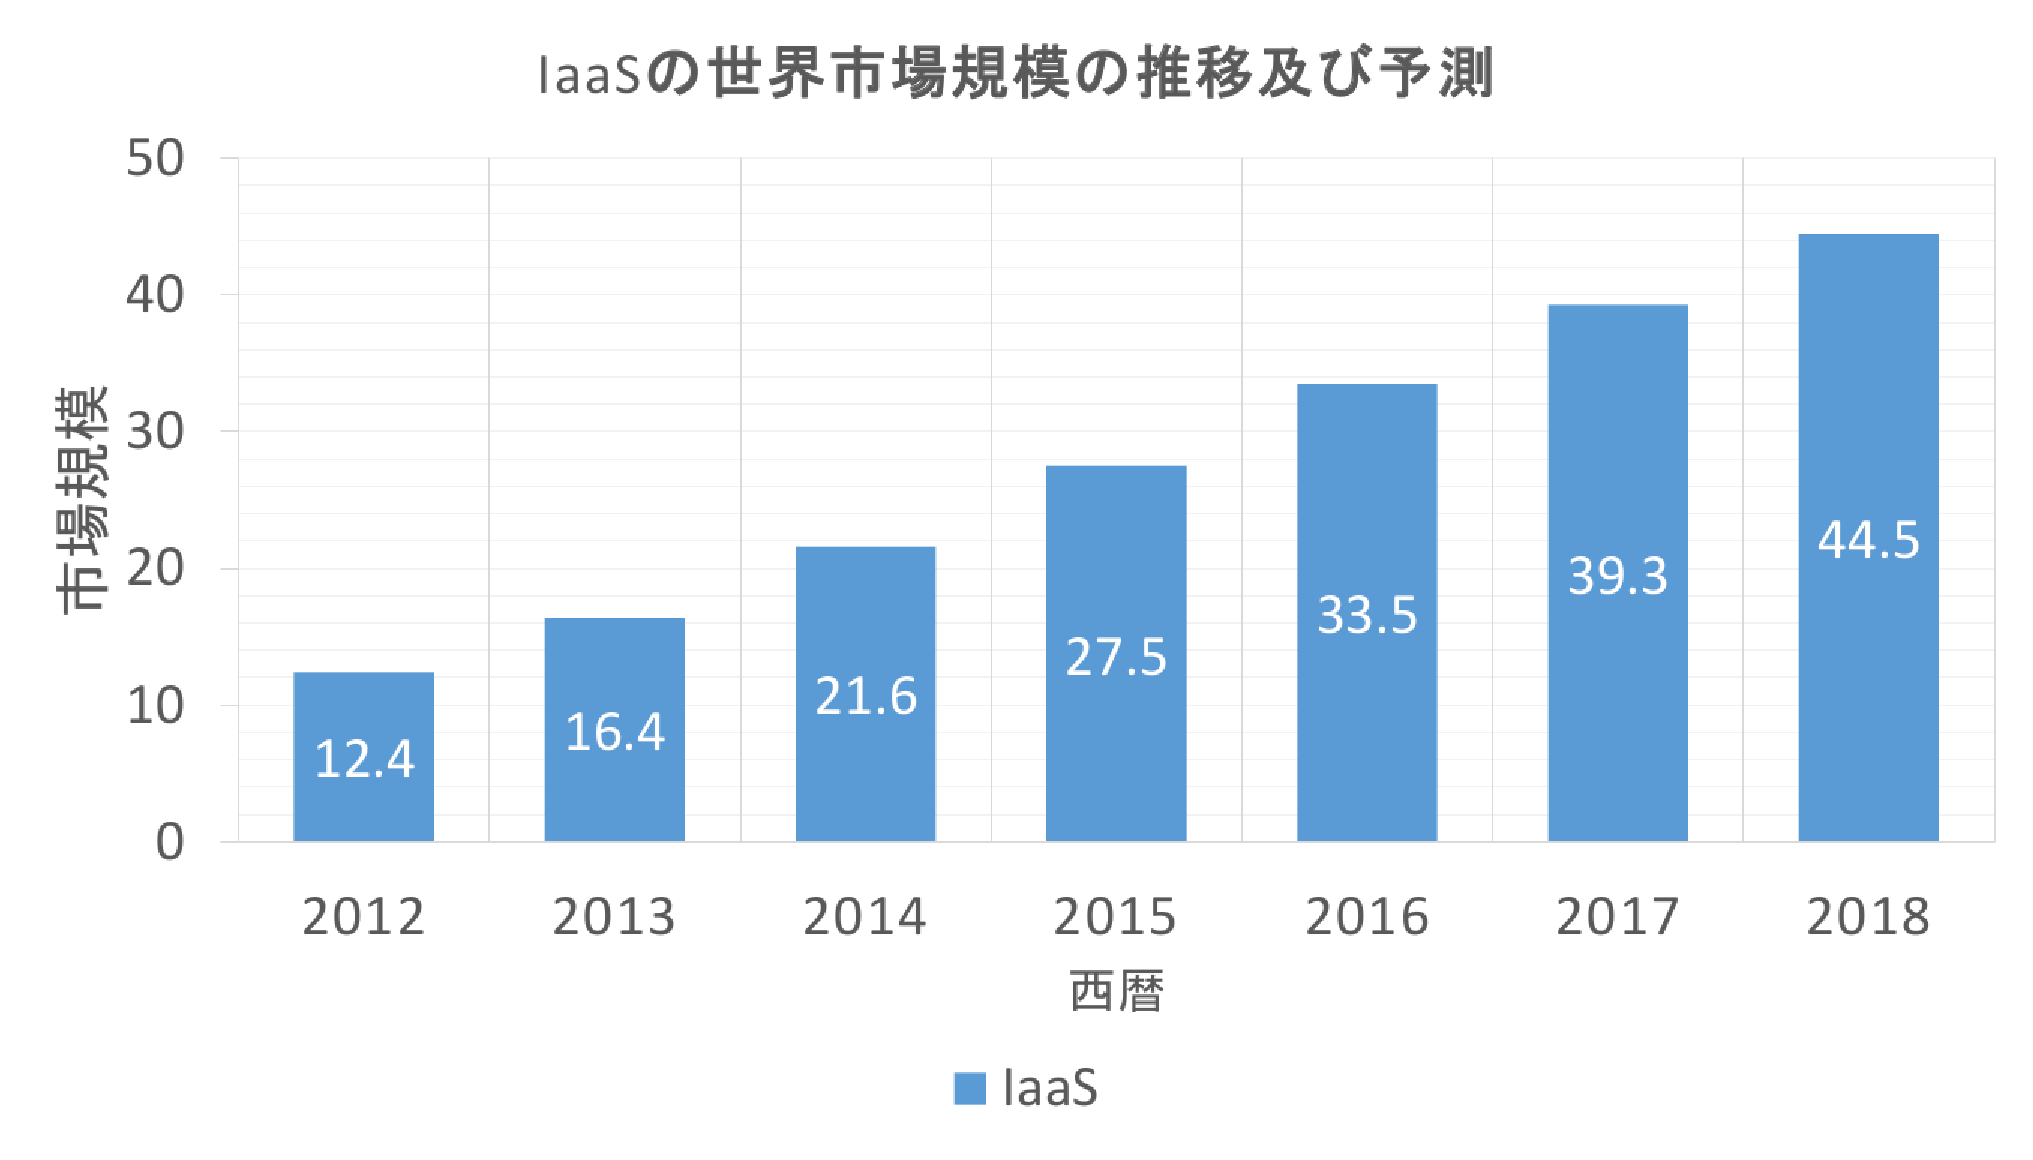
\includegraphics[scale=0.4]{Document/IaaSGrafNew.eps}
			\caption{クラウドサービスの世界市場規模の推移及び予測}
			\label{graf:1}
		\end{center}
	\end{figure}
	
	IaaS(Infrastructure as a Service)とは,システムの稼働に必要なサーバー,ストレージ,ネットワークなどのインフラを,ネットワーク経由で提供するサービスのことである.\cite{bib:2}IaaSを提供する側は物理サーバーや物理ネットワークを仮想化しIaaS基盤を構築してサービスを提供する.IaaSを提供される側は,仮想化されたリソースを組み合わせシステムを構築,サービスを提供させることが可能となる.
	IaaSの代表的なサービスとして,「Amazon Web Services」や,「Microsoft Azure」等が挙げられる.これらのサービスは,提供しているベンダが1つであり,それぞれ独自仕様で開発されたIaaS基盤を用いている.
	
	それに対し,多くのベンダが参加するコミュニティで開発されているIaaS基盤構築ソフトウェアとしてOpenStackが存在する.\cite{bib:3}OpenStackはオープンソース・ソフトウェアとして開発されており,Amazon Web Service や Microsoft Azure と違い独自仕様で開発されていない.コミュニティに参加している企業は,オープンソース・ソフトウェアとして開発されたOpenStackをベースとしてIaaSを提供している.
	
	OpenStackは,2010年10月に初期バージョンであるAustinがリリースされ,その後定期的に新しいバージョンを公開した後,2015年10月16日に最新バージョンのLibertyが公開されている.機能別にコンポーネントが分かれており,各コンポーネントが相互に連携して動作する.OpenStackの主要コンポーネントを表\ref{table:1}に示す.
	\begin{table}[H]
		\begin{center}
			\caption{OpenStackの主要コンポーネント}
			\label{table:1}
			\begin{tabular}{|c|c|}\hline
				コンポーネント & 機能\\ \hline \hline
	     		Glance & 仮想マシンで使用されるゲストOSの管理\\ \hline
				Cinder & ブロックストレージにてゲストOS等を永続管理\\ \hline
				Neutron & 仮想ネットワークの管理\\ \hline
				Horizon & OpenStackの操作管理を行うWebUIの提供\\ \hline
				Swift & オブジェクトストレージの提供\\ \hline
				Heat & 仮想環境構築のためのオーケストレーション機能の提供\\ \hline
			\end{tabular}
		\end{center}
	\end{table}
	Heatとは,本来OpenStack利用者が手動で,各コンポーネントに指示を出し行っている仮想環境構築の手順を自動化する機能を提供している.自動化の手順としては,各コンポーネントを実行するために必要な項目を「Heatテンプレートファイル(以降テンプレートファイルと呼ぶ)」に記述後,テンプレートファイルを読み込むことで各コンポーネントで実行される内容を定義した後,自動で実行し仮想環境を構築を行うというものである.尚,テンプレートファイルには独自の書式が存在する.\cite{bib:4}
	
	OpenStackの各コンポーネントを自動化することができるHeatだが,現状問題が存在する.図\ref{table:2}に問題点を示す.
	
	\begin{table}[H]
		\begin{center}
			\caption{Heatの問題点}
			\label{table:2}
			\begin{tabular}{|p{5cm}|p{7cm}|}\hline
				問題点 & 詳細\\ \hline \hline
				テンプレートファイルから構成情報を把握しづらい & 構成情報を全てテキストで記述しているため,一見して構築途中または構築完了後の構成をテンプレートファイルからは把握しづらい.\\ \hline
				テンプレートファイルの書式が複雑 & 入力内容を把握しづらい.どのコンポーネントへ命令を出すか,また各コンポーネント内で分岐している命令文の選択も複雑な書式といえる.また,文中のインデントの深さで入力内容を区別するという特殊な書式もある.\\ \hline
				膨大なテキスト記述量 & 手動入力で仮想環境のシステム構成について記述するため,記述に膨大な時間がかかる.\\ \hline
			\end{tabular}
		\end{center}
	\end{table}
% %	\begin{itemize}
	% %	\item Heatテンプレートファイルの複雑な書式
	% %	\begin{itemize}
		% %	\item 入力内容の不明確さ
		% %	\item インデントの深さによる入力項目区別
		% %\end{itemize}
		% %\item テキスト記述量
		% %\begin{itemize}
		% %	\item 新規項目追加毎に関連項目全てを追加入力
		% %\end{itemize}
		% %\item テンプレートファイルから構成情報を把握することの難しさ
		% %\begin{itemize}
		% %	\item 複雑な書式,膨大な量のテキスト記述量から一見して構成を把握することが困難
		% %\end{itemize}
	% %\end{itemize}
% %	提示した問題点を解決するために,以下の解決案を提案する.
	% %\begin{itemize}
	% %	\item Heat専門知識の排除
	% % % %	\item 入力者側が細かな書式を気にしないで済むようなもの
	% %	\end{itemize}
	% %	\item 入力内容の明確化
	% %	\begin{itemize}
	% %		\item 何を入力すればよいのか項目名を追加
	% %	\end{itemize}
	% % 	\begin{itemize}
	% %		\item インスタンス名記述項目以外の項目で手動入力を撤廃,プルダウンメニューによる選択肢を提供
	% %	\end{itemize}
	% %	\item 構成情報の可視化
	% %	\begin{itemize}
	% %		\item 現在構築中の構成情報についてアイコンを用いて可視化
	% %	\end{itemize}
% %	\end{itemize}
	
	
\chapter{オーケストレーション定義エディタの提案}
%\input{chpater2.tex}
	\section{オーケストレーション定義エディタの概要}
		オーケストレーション定義エディタとは,従来手動で行っていたテンプレートファイル作成をGUIベースで作成補助をすることによりテンプレートファイル作成にかかる時間を削減し,容易にHeatを用いた仮想環境構築を可能にするエディタである.オーケストレーション定義エディタの概略図を図\ref{graf:2}に示す.
		\vspace{-2mm}
		\begin{figure}[H]
			\begin{center}
				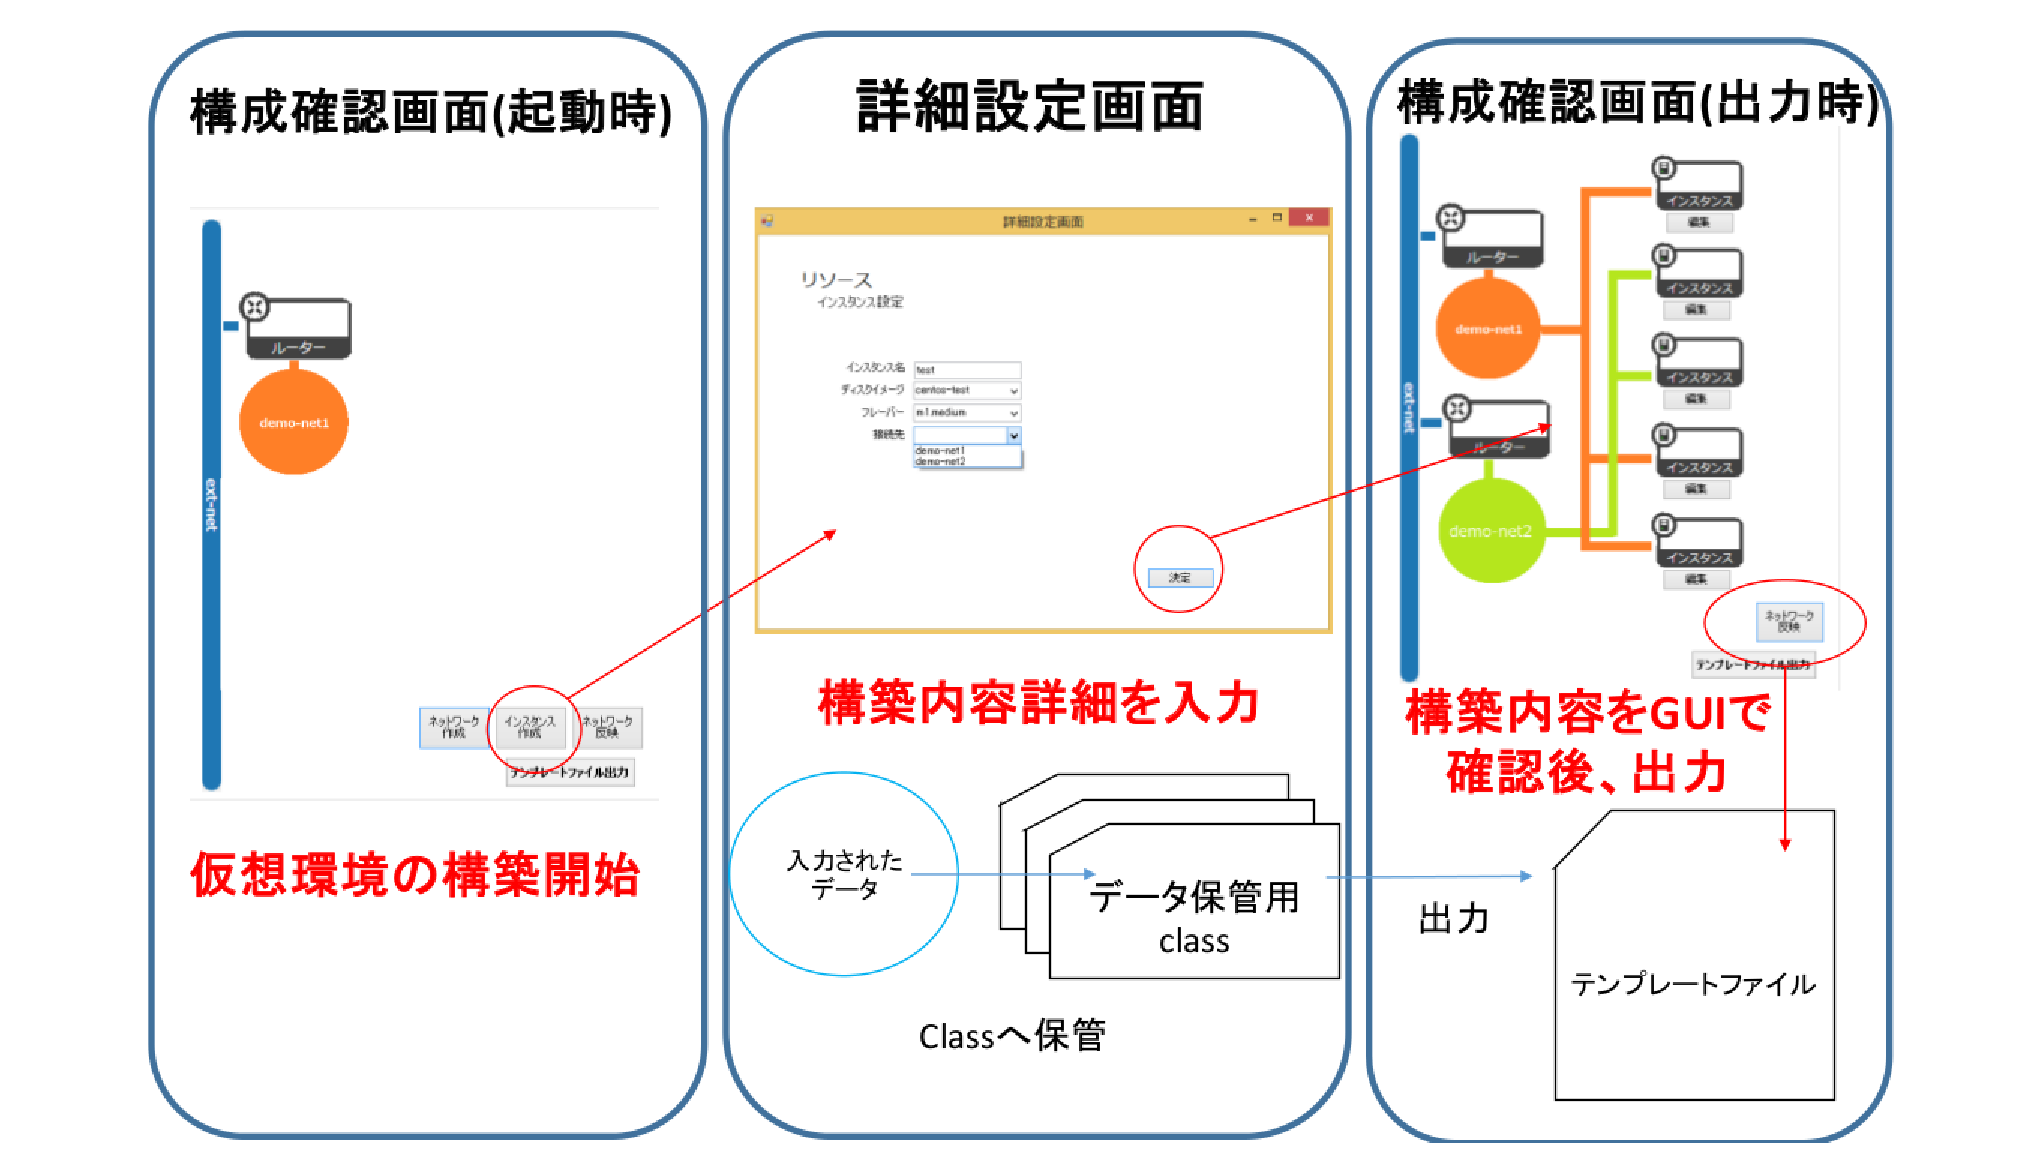
\includegraphics[scale=0.4]{Document/GUIEditorOverview.eps}
				\caption{オーケストレーション定義エディタの概略}
				\label{graf:2}
			\end{center}
		\end{figure}
	\section{オーケストレーション定義エディタの要件}
	オーケストレーション定義エディタで取り扱うHeatはOpenStack内のコンポーネントであるため利用者はHeatを使用する際にはOpenStackについての最低限必要な知識を身に着けている必要がある.それ以外の前提知識を身につけていなくとも利用者がスムーズに仮想環境を構築するために表\ref{table:3}にオーケストレーション定義エディタに求められる要件を定義した.
	\begin{table}[H]
		\begin{center}
			\caption{オーケストレーション定義エディタに求められる要件}
			\label{table:3}
			\begin{tabular}{|p{5cm}|p{7cm}|}\hline
				要件 & 理由\\ \hline \hline
				操作インターフェイスはGUI & 構築中のシステム構成を可視化するため\\ \hline
				利用対象者はOpenStackに関する基本的な知識を有した学生 & HeatはOpenStack内のコンポーネントであり,OpenStack内GUIであるDashboardの利用者の多くは学生以上であるため\\ \hline
				%扱うシステム構成のネットワーク規模は1から3セグメント & (まだ理由がない)\\ \hline
				インスタンス名入力項目以外の手動入力方式を廃止 & テキスト入力量を削減し,テンプレートファイル作成にかかる時間を短縮するため\\ \hline
				入力項目の明確化 & 予め正しい入力内容へ誘導することで,テンプレートファイル読み込み時のエラーを抑止\\ \hline
			\end{tabular}
		\end{center}
	\end{table}
	\section{Heatで扱うリソース}
	オーケストレーション定義を行うHeatでは,複数個のリソースを取り扱っている.お互いに依存しあうリソースについて記述を行うことで仮想環境を構築する.
	
	\subsection{リソースの依存関係}
	Heatで取り扱うリソースはそれぞれ他のリソースに依存している.依存しているリソースを参照することで仮想環境を稼働させる.依存関係を表\ref{table:4}と図\ref{graf:7}に示す.
	\begin{table}[H]
		\begin{center}
			\caption{リソースの依存関係表}
			\label{table:4}
			\begin{tabular}{|p{5cm}|p{7cm}|}\hline
				リソース & 依存している他のリソース\\ \hline \hline
				ネットワーク及びサブネット & 外部へ接続する必要があるため,外部ネットワークを参照する.サブネットでは使用するIPアドレス範囲を指定.\\ \hline
				ルーター & 接続先を指定するためにネットワークを参照する.\\ \hline
				ルーターインターフェイス & ネットワークとルータを接続している.どのネットワークが自身の依存するルータに接続されるのか管理している.\\ \hline
				インスタンス & 接続先を指定するためにネットワークを参照している.参照したネットワークに応じて,予めサブネットで範囲指定しておいたIPアドレスを割り振り,ルータを介して外部ネットワークへ接続できる.\\ \hline
			\end{tabular}
		\end{center}
	\end{table}
	
	\begin{figure}[H]
		\begin{center}
			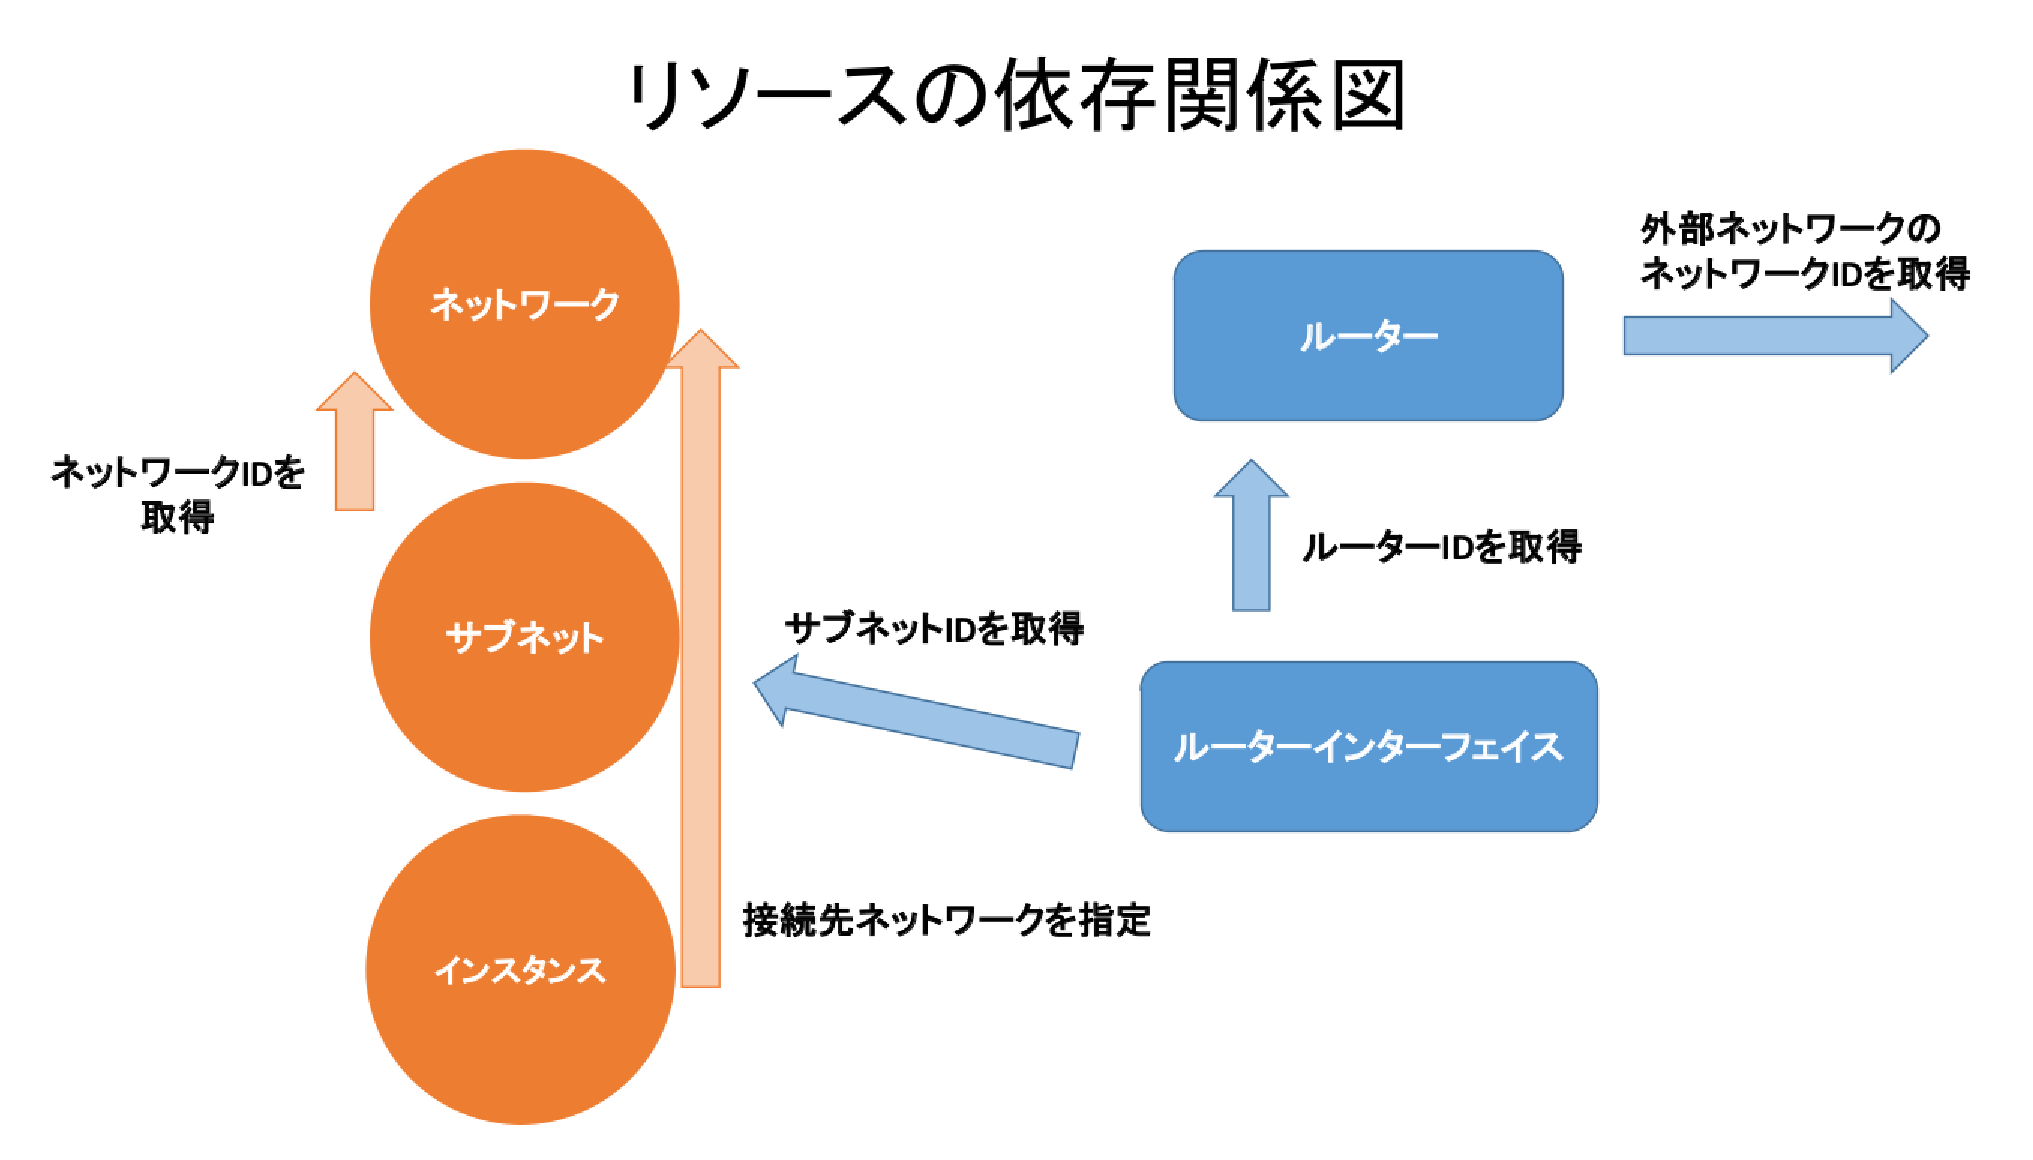
\includegraphics[scale=0.45]{Document/ResourcesRelational.eps}
			\caption{リソースの依存関係図}
			\label{graf:7}
		\end{center}
	\end{figure}
	
	
	構成上最も外側のネットワークを参照できるのは内部に存在するネットワークである.外のネットワークへの出口を確保することで,セグメント内から外部へネットワークを通じて接続できるようにしている.サブネットではセグメント内で使用するIPアドレスの幅を設定する.ここで設定されたIPアドレス範囲内にインスタンスを接続する.
	
	Heatでは,これらリソースの依存関係,参照先をテンプレートファイルへ記述後,テンプレートを読み込むことで自動で仮想環境を構築する.
	\section{テンプレートファイルへの出力補助方法}
	仮想環境構築を補助するHeatだが,テンプレートファイル作成には多大な時間がかかり,更には記述の為にHeatに関する専門知識が必要であるため手軽に利用できない.そこでテンプレートファイル作成を容易にするため,オーケストレーション定義エディタではテンプレートファイルへの出力補助を行う.
	
	オーケストレーション定義エディタでは,ユーザに入力されたデータは一度「データ保管用Class」へ保管する.(図\ref{graf:3})このデータ保管用Classにはオーケストレーション定義エディタからであれば何度もアクセスと編集が可能である.そのため構築途中で既に記述をした項目を修正することも容易である.入力された複数のデータをデータ保管用Classに保持し続けておき,テンプレートファイルへ出力を行う際にデータ保管用Classを呼び出しClass内に保管されているデータをテンプレートファイルへ出力する.
	
	\begin{figure}[H]
		\begin{center}
			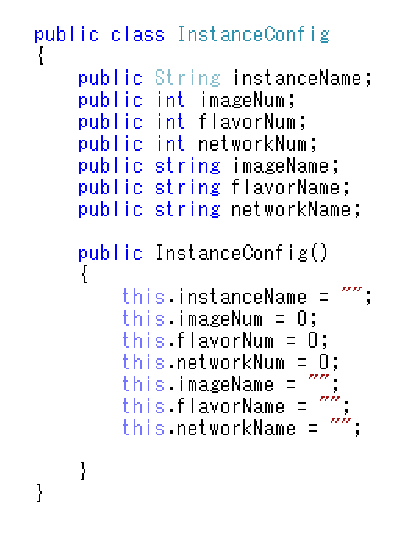
\includegraphics[scale=1.3]{Document/Source1.eps}
			\caption{データ保管用Class}
			\label{graf:3}
		\end{center}
	\end{figure}
	
\chapter{オーケストレーション定義エディタの実装}
	\section{動作環境}
	本研究で作成されたオーケストレーション定義エディタはプログラミング言語であるC\#を使用して作成されているので,動作には「Microsoft .NET Framework 4.6」環境が必要である.
	\section{画面構成}
	オーケストレーション定義エディタは\ref{graf:2}の概略図で示したとおり,大きく分けて2つの画面から構成されている.オーケストレーション定義エディタに表示される「構成確認画面」と呼ばれる画面と,構成確認画面内から遷移できる「詳細設定画面」という画面である.以下に各画面の詳細を示す.
	\newpage
		\subsection{構成確認画面}
		構成確認画面では,これから構築する構成をGUIベースで確認することが可能である.図\ref{pic:1}に示す通り,オーケストレーション定義エディタ起動時には予め1セグメントのみ準備されている.これは,仮想環境を構築するのであれば最低1セグメントはネットワークが必要だからである.1セグメント目のネットワークに関する記述はどの構成でも必要な記述であるため,予めオーケストレーション定義エディタの構成確認画面ではルーターとネットワークを作成済みの状態で起動される.
		
		\begin{figure}[h]
			\begin{center}
				\includegraphics[scale=0.55]{Document/構成確認画面1.eps}
				\caption{オーケストレーション定義エディタ-構成確認画面その1}
				\label{pic:1}
			\end{center}
		\end{figure}
		オーケストレーション定義エディタ起動時の画面を図\ref{pic:2}に示す.1セグメント目のルーターとネットワーク以外にセグメントを増やしたい場合は,画面下部のネットワーク作成ボタンを押すことで次のセグメントを追加する.追加されたネットワークは,接続先ネットワークとして詳細入力画面から参照可能となる.
		\begin{figure}[H]
			\begin{center}
				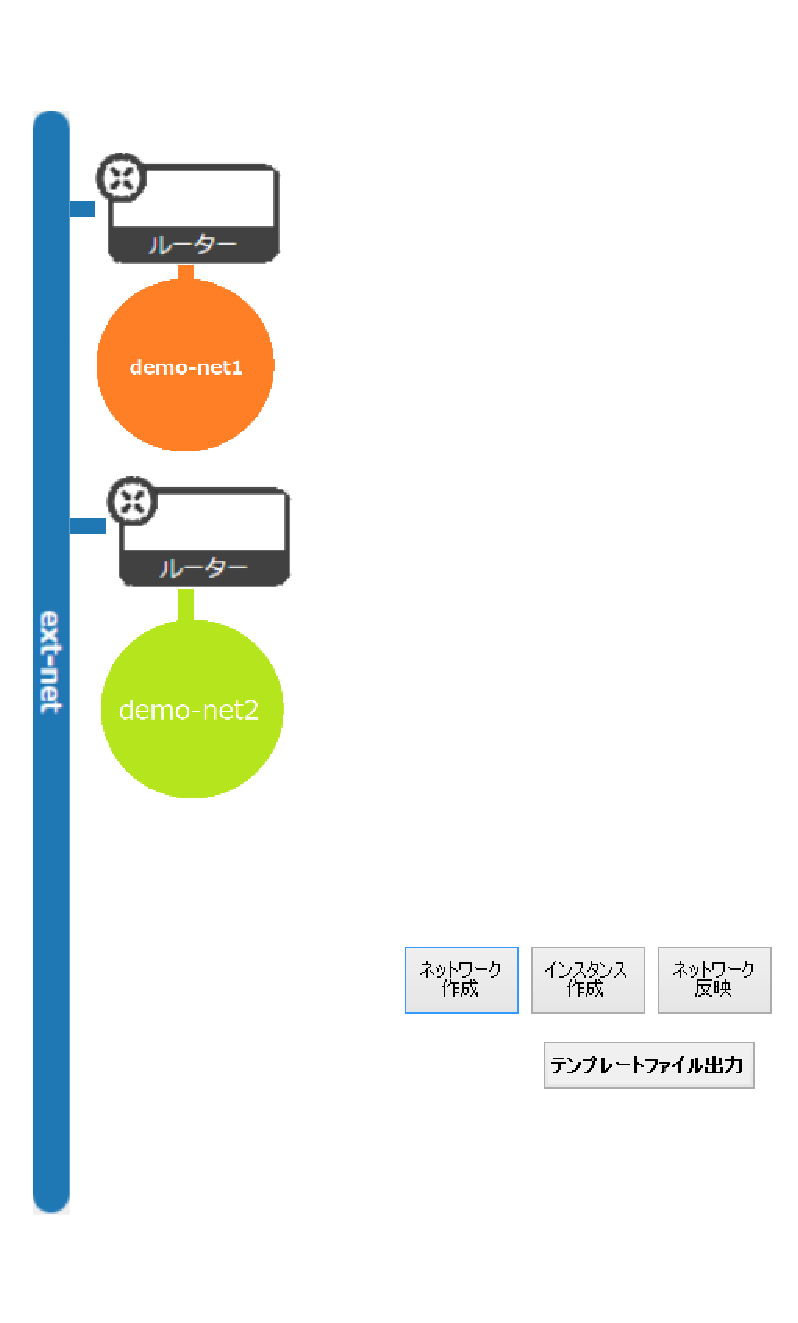
\includegraphics[scale=0.55]{Document/構成確認画面2.eps}
				\caption{オーケストレーション定義エディタ-構成確認画面その2}
				\label{pic:2}
			\end{center}
		\end{figure}
		インスタンスを作成したい場合は,画面下部のインスタンス作成ボタンを押すことで新規作成するインスタンスを追加できる.ただしここで作成ボタンを押しただけではインスタンスに関する詳細設定ができていない状態であるため,作成後はインスタンスアイコンの下部にある編集ボタンをクリックして詳細入力画面に遷移しなければならない.尚,詳細設定画面で項目を入力した後構成確認画面に戻り画面下部のネットワーク反映ボタンを押すと,図\ref{pic:3}のようにGUIで接続先が把握できる.
		\begin{figure}[H]
			\begin{center}
				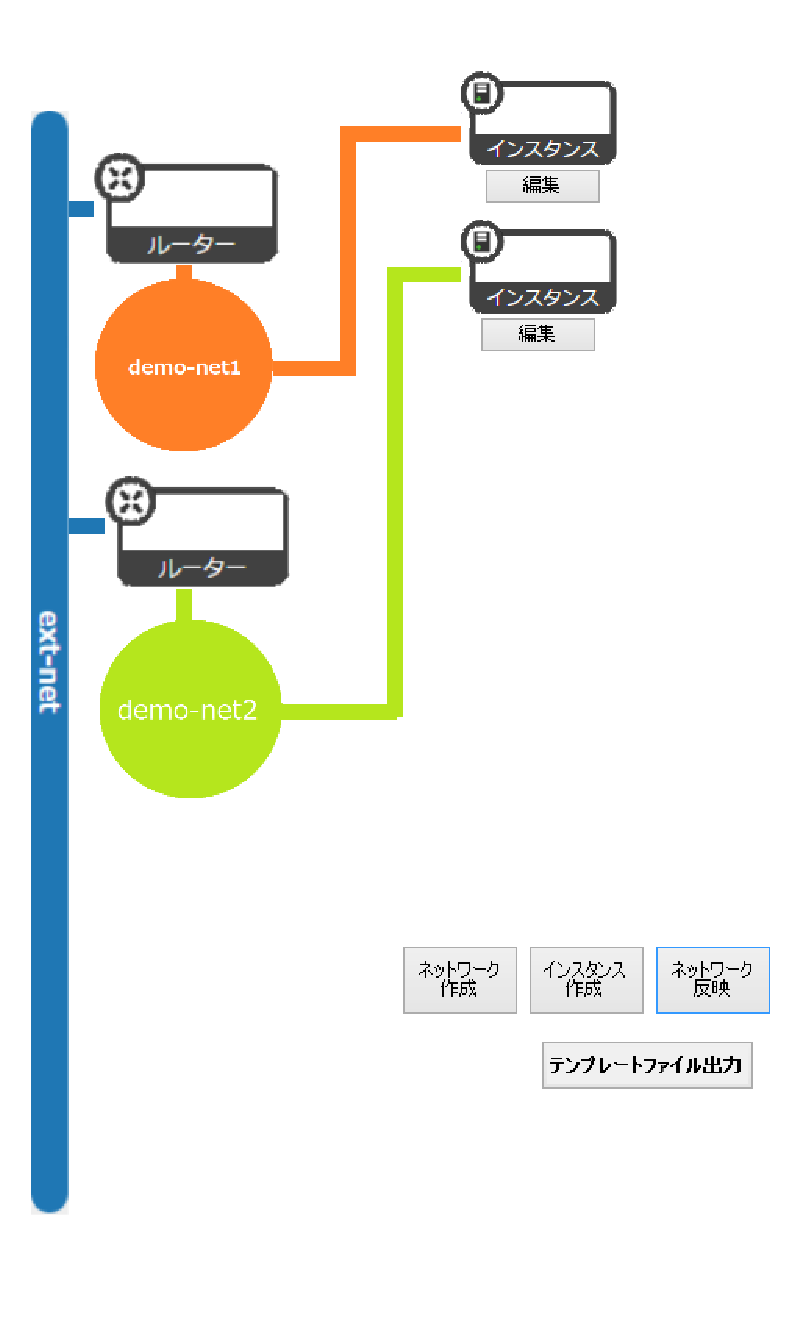
\includegraphics[scale=0.55]{Document/構成確認画面3.eps}
				\caption{オーケストレーション定義エディタ-構成確認画面その3}
				\label{pic:3}
			\end{center}
		\end{figure}
		
		また,図\ref{pic:3}のように構成内容を決定した後でも,オーケストレーション定義エディタを終了させなければ構成内容の編集が可能である.図\ref{pic:3}の状態から一度インスタンスの接続先ネットワークを変更,作成するネットワークとインスタンスを増加させることも可能であり,図\ref{pic:5}と図\ref{pic:6}のように遷移する.
		\begin{figure}[H]
			\begin{center}
				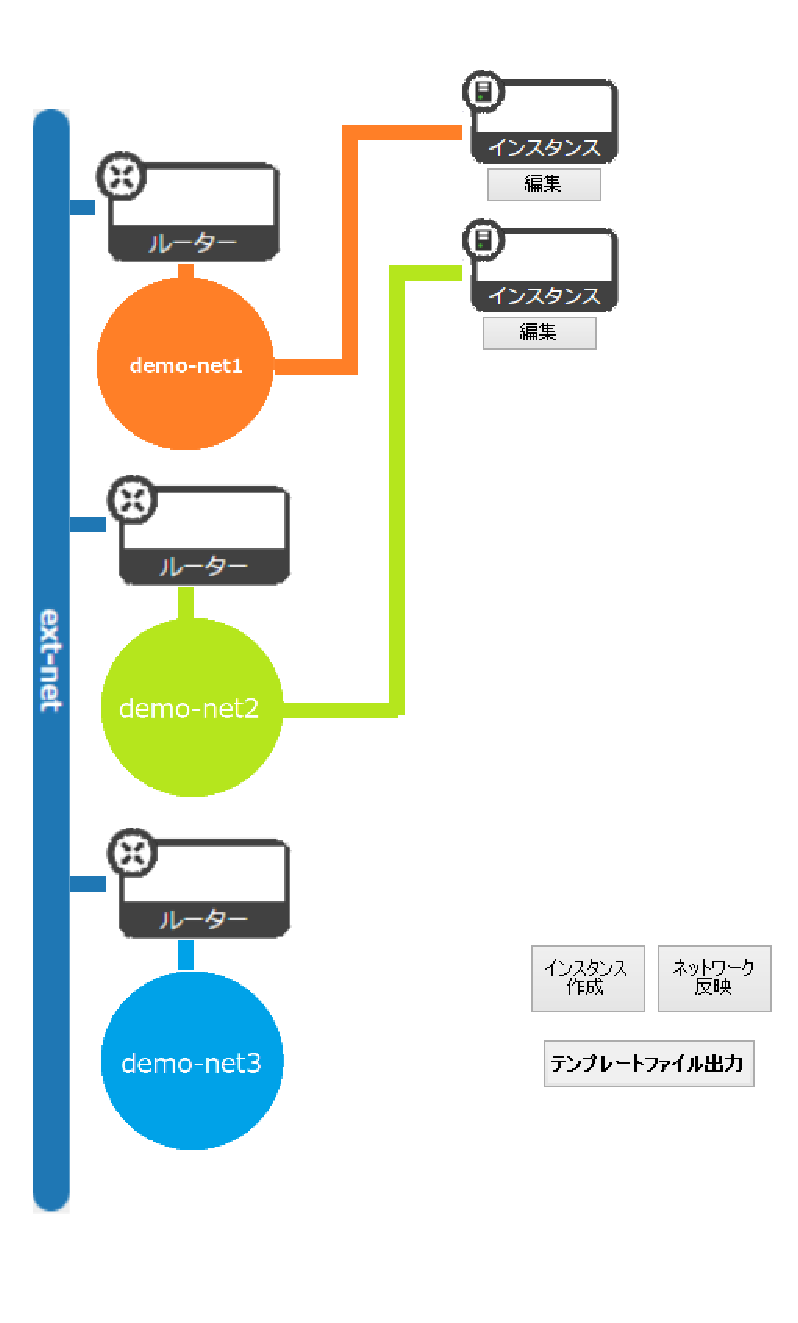
\includegraphics[scale=0.55]{Document/構成確認画面ex1.eps}
				\caption{オーケストレーション定義エディタ-構成確認画面その4}
				\label{pic:5}
			\end{center}
		\end{figure}
		
		\begin{figure}[H]
			\begin{center}
				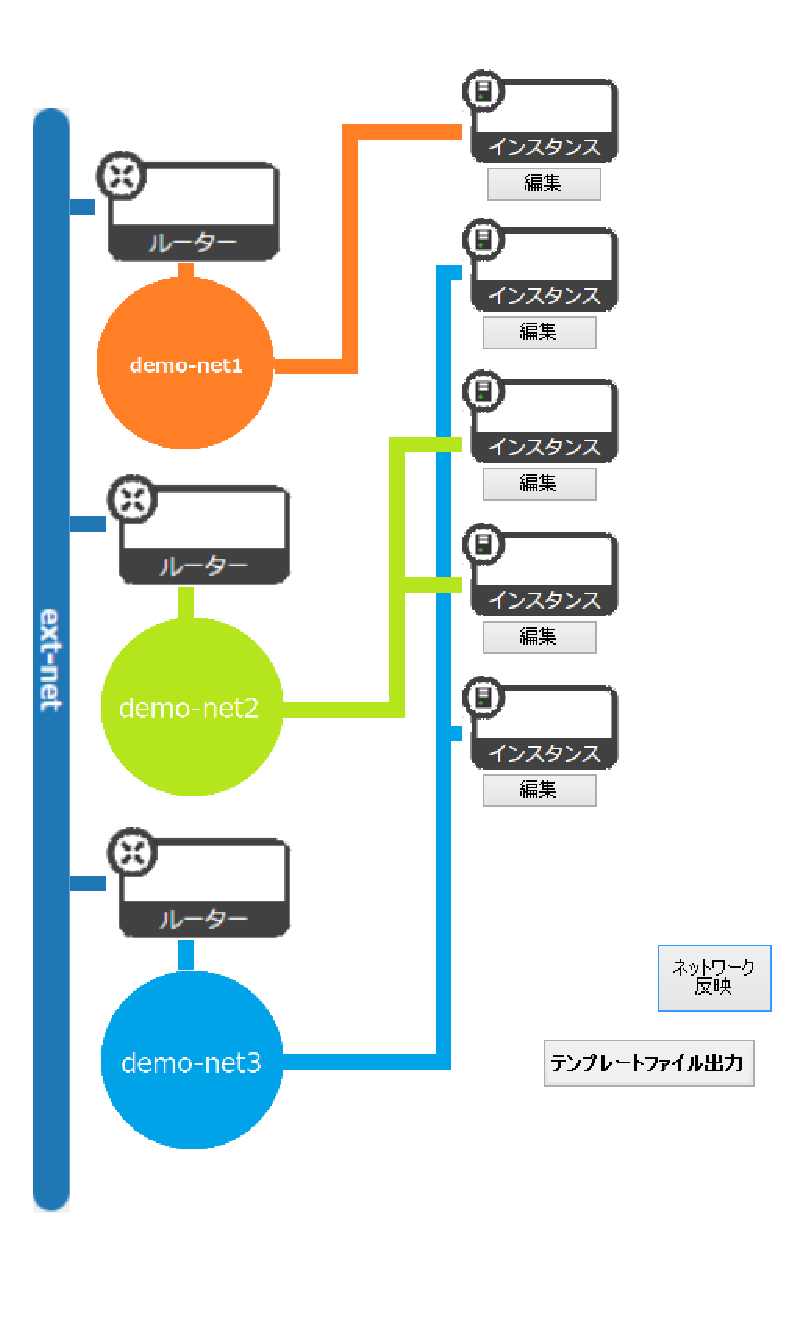
\includegraphics[scale=0.55]{Document/構成確認画面ex2.eps}
				\caption{オーケストレーション定義エディタ-構成確認画面その5}
				\label{pic:6}
			\end{center}
		\end{figure}
		
		
		\subsection{詳細入力画面}
		インスタンスに関する詳細入力は,構成確認画面から遷移できる詳細入力画面で行う.詳細入力画面の様子を図\ref{pic:4}に示す.詳細入力画面で入力できる4つの項目のうちインスタンス名を入力する項目1つを除き全てプルダウンメニューを採用している.インスタンス名のみ,自由に入力できる項目であるため手動入力形式であるが,その他3つの項目はある程度入力される内容が決まっているがインスタンス毎に入力内容が違う可能性がある.そこで選択肢を提供するためにプルダウンメニューを採用した.尚,構成確認画面でネットワークを追加した場合は「接続先」項目の選択肢が自動で追加される.
		
			\begin{figure}[H]
				\begin{center}
					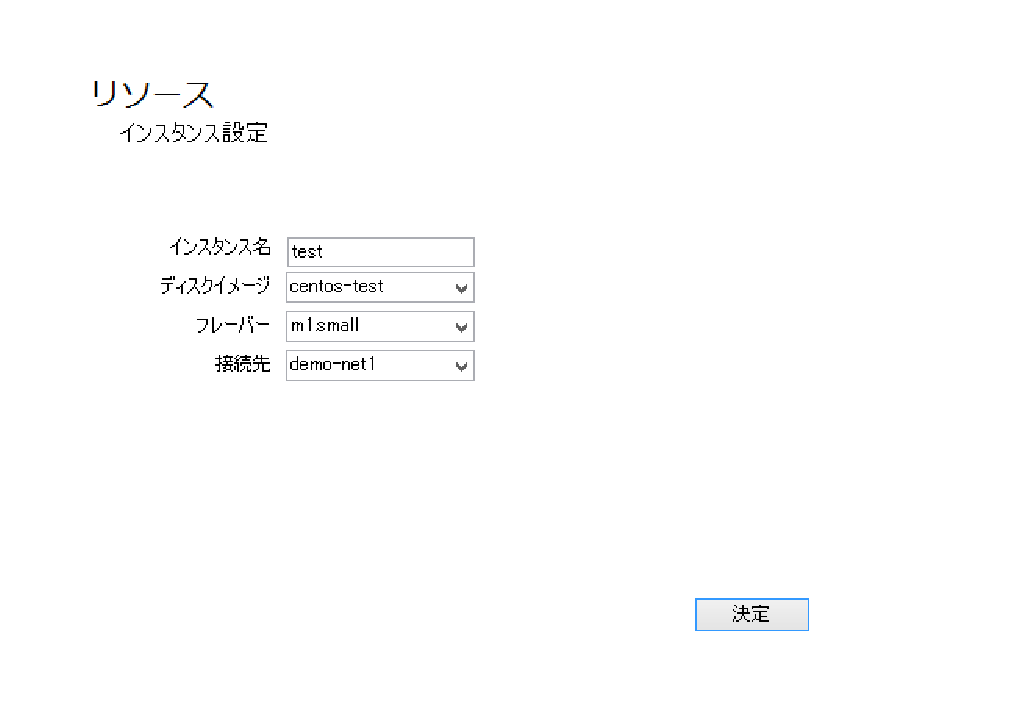
\includegraphics[scale=1.1]{Document/詳細設定画面.eps}
					\caption{オーケストレーション定義エディタ-詳細設定画面}
					\label{pic:4}
				\end{center}
			\end{figure}
	\section{テンプレートファイル出力の流れ}
	オーケストレーション定義エディタで受け付けた入力内容は最終的にテンプレートファイルへと出力される.
		\subsection{ネットワークに関する記述}
		ネットワークに関する記述である,ネットワークについての記述,サブネットについての記述,ルーターについての記述,ルーターインターフェイスは構成確認画面での入力内容に応じて記述内容が変化する.構成確認画面でネットワークに対して行える操作は,新たなネットワークの追加のみである.
		
		その他ネットワークに関する細かな記述は,記述量こそ多いが依存・参照するものが決まっているので,予め文字列データとして保存しておき,必要な箇所へ自動で出力される.
		\subsection{インスタンスに関する記述}
		インスタンスに関する記述である,インスタンス名,ディスクイメージ,フレーバー,接続先ネットワーク名は図\ref{graf:3}で示したデータ保管用Classへ一度保管される.その後ファイル出力時にテンプレートファイルへ出力される.
\chapter{評価}
	\section{評価の目的}
	1章「はじめに」中で提示した「Heatの問題点」を解決できたか検証,従来方式との差を計測するために被験者の,各手法に関する前提知識の勉強時間,作成インスタンス数とルーター数の増加させての作成所要時間,テンプレートファイル読み込み時にチェックされる記述ミスによるエラー発生数を計測,従来方式とオーケストレーション定義エディタ使用時それぞれで同じシステム構成を構築してもらい比較する.
	\section{評価内容}
	従来方式,オーケストレーション定義エディタそれぞれでシステム構築をする場合に以下の表\ref{table:5}に示している評価要素についてデータを記録する.
	\begin{table}[H]
		\begin{center}
			\caption{評価要素}
			\label{table:5}
			\begin{tabular}{|p{5cm}|p{7cm}|}\hline
				評価要素 & 詳細\\ \hline \hline
				学習時間 & 各方式についての前提知識を説明用ドキュメントを用いて学習するのにかかった時間\\ \hline
				作成所要時間 & 各方式それぞれテンプレートファイル作成開始からテンプレートファイルをエラー無しの状態で正常に読み込ませるまでに要した時間\\ \hline
				エラー発生回数 & テンプレートファイルをHeatに読み込ませた時にエラーが発生した回数.正常に読み込み完了となるまで修正したテンプレートファイルを読みこませ直し続けるのでその都度エラーが発生すればカウントする\\ \hline
			\end{tabular}
		\end{center}
	\end{table}
	\section{評価環境}
	本評価実験は,オーケストレーション定義エディタの動作環境を満たしている「Microsoft .NET Framework 4.6」環境で評価を行った.
	
	また,本評価実験で構築する仮想環境システム構成を以下に示す.
	\begin{description}
		\item [I.(1セグメント1インスタンス構成)]\mbox{}\\ 作成するネットワーク(ルーター)数は1,インスタンス数も1.
		\item [I\hspace{-1pt}I.(1セグメント3インスタンス構成)]\mbox{}\\ 作成するネットワーク(ルーター)数は1,インスタンス数は3.
		\item [I\hspace{-1pt}I\hspace{-1pt}I.(1セグメント5インスタンス構成)]\mbox{}\\ 作成するネットワーク(ルーター)数は1,インスタンス数は5.
		\item [I\hspace{-1pt}V.(2セグメント5インスタンス構成)]\mbox{}\\ 作成するネットワーク(ルーター)数は2,インスタンス数は5.
		\item [V.(3セグメント5インスタンス構成)]\mbox{}\\ 作成するネットワーク(ルーター)数は3,インスタンス数は5.
	%	\item instance数3つ,Router数1つ
	%	\item instance数5つ,Router数1つ
	%	\item instance数5つ,Router数2つ
	%	\item instance数5つ,Router数3つ
	\end{description}
	
	I,I\hspace{-1pt}I,I\hspace{-1pt}I\hspace{-1pt}I 3つの構成は単純にインスタンスの数のみを増加させ,残るI\hspace{-1pt}V,V のシステム構成は基本的な構成はI\hspace{-1pt}I\hspace{-1pt}Iと同じだが,作成するルーターの数(内部のネットワーク,サブネットの数)を増加させている.これは,インスタンスに関する記述のみを増加させた場合とルーターに関する記述を増加させた場合,記述増加量の差があるため双方の記述所要時間とエラー発生回数の増加幅やデータの動きに差が生まれると予測したためである.
	\section{結果}
	評価実験の結果を,従来方式については表\ref{table:6},オーケストレーション定義エディタについては表\ref{table:7}に示す.
	
	\begin{table}[H]
		\begin{center}
				\vspace{-4mm}
			\caption{各評価要素の実験結果-従来方式}
			\label{table:6}
			\begin{tabular}{|p{3cm}|p{2cm}|p{2cm}|}\hline
				評価要素 & 最小値 & 最大値\\ \hline \hline
				学習時間 & 413(秒) & 540(秒)\\ \hline
				作成所要時間 (I) & 685(秒) & 1328(秒)\\ \hline
				作成所要時間 (I\hspace{-1pt}I) & 531(秒) & 1560(秒)\\ \hline
				作成所要時間 (I\hspace{-1pt}I\hspace{-1pt}I) & 597(秒) & 931(秒)\\ \hline
				作成所要時間 (I\hspace{-1pt}V) & 525(秒) & 1258(秒)\\ \hline
				作成所要時間 (V) & 485(秒) & 1532(秒)\\ \hline
				エラー発生回数 (I) & 1(回) &  7(回)\\ \hline
				エラー発生回数 (I\hspace{-1pt}I) & 1(回) &  3(回)\\ \hline
				エラー発生回数 (I\hspace{-1pt}I\hspace{-1pt}I) & 0(回) &  5(回)\\ \hline
				エラー発生回数 (I\hspace{-1pt}V) & 0(回) &  7(回)\\ \hline
				エラー発生回数 (V) & 0(回) &  4(回)\\ \hline
			\end{tabular}
		\end{center}
	\end{table}
	
	\begin{table}[H]
		\begin{center}
			\vspace{-4mm}
			\caption{各評価要素の実験結果-オーケストレーション定義エディタ}
			\label{table:7}
			\begin{tabular}{|p{3cm}|p{2cm}|p{2cm}|}\hline
				評価要素 & 最小値 & 最大値\\ \hline \hline
				学習時間 & 72(秒) & 180(秒)\\ \hline
				作成所要時間 (I) & 27(秒) & 71(秒)\\ \hline
				作成所要時間 (I\hspace{-1pt}I) & 87(秒) & 166(秒)\\ \hline
				作成所要時間 (I\hspace{-1pt}I\hspace{-1pt}I) & 105(秒) & 190(秒)\\ \hline
				作成所要時間 (I\hspace{-1pt}V) & 113(秒) & 228(秒)\\ \hline
				作成所要時間 (V) & 142(秒) & 229(秒)\\ \hline
				エラー発生回数 (I) & 0(回) &  0(回)\\ \hline
				エラー発生回数 (I\hspace{-1pt}I) & 0(回) &  0(回)\\ \hline
				エラー発生回数 (I\hspace{-1pt}I\hspace{-1pt}I) & 0(回) &  0(回)\\ \hline
				エラー発生回数 (I\hspace{-1pt}V) & 0(回) &  0(回)\\ \hline
				エラー発生回数 (V) & 0(回) &  0(回)\\ \hline
			\end{tabular}
		\end{center}
	\end{table}
	\section{考察}
	\begin{description}
		\item[(学習時間について)]\mbox{}\\  従来方式,オーケストレーション定義エディタ双方の学習時間を比較すると,全ての被験者がオーケストレーション定義エディタについての学習時間が従来方式よりも短いことがわかる.(図\ref{graf:8})
		
			\begin{figure}[H]
				\begin{center}
					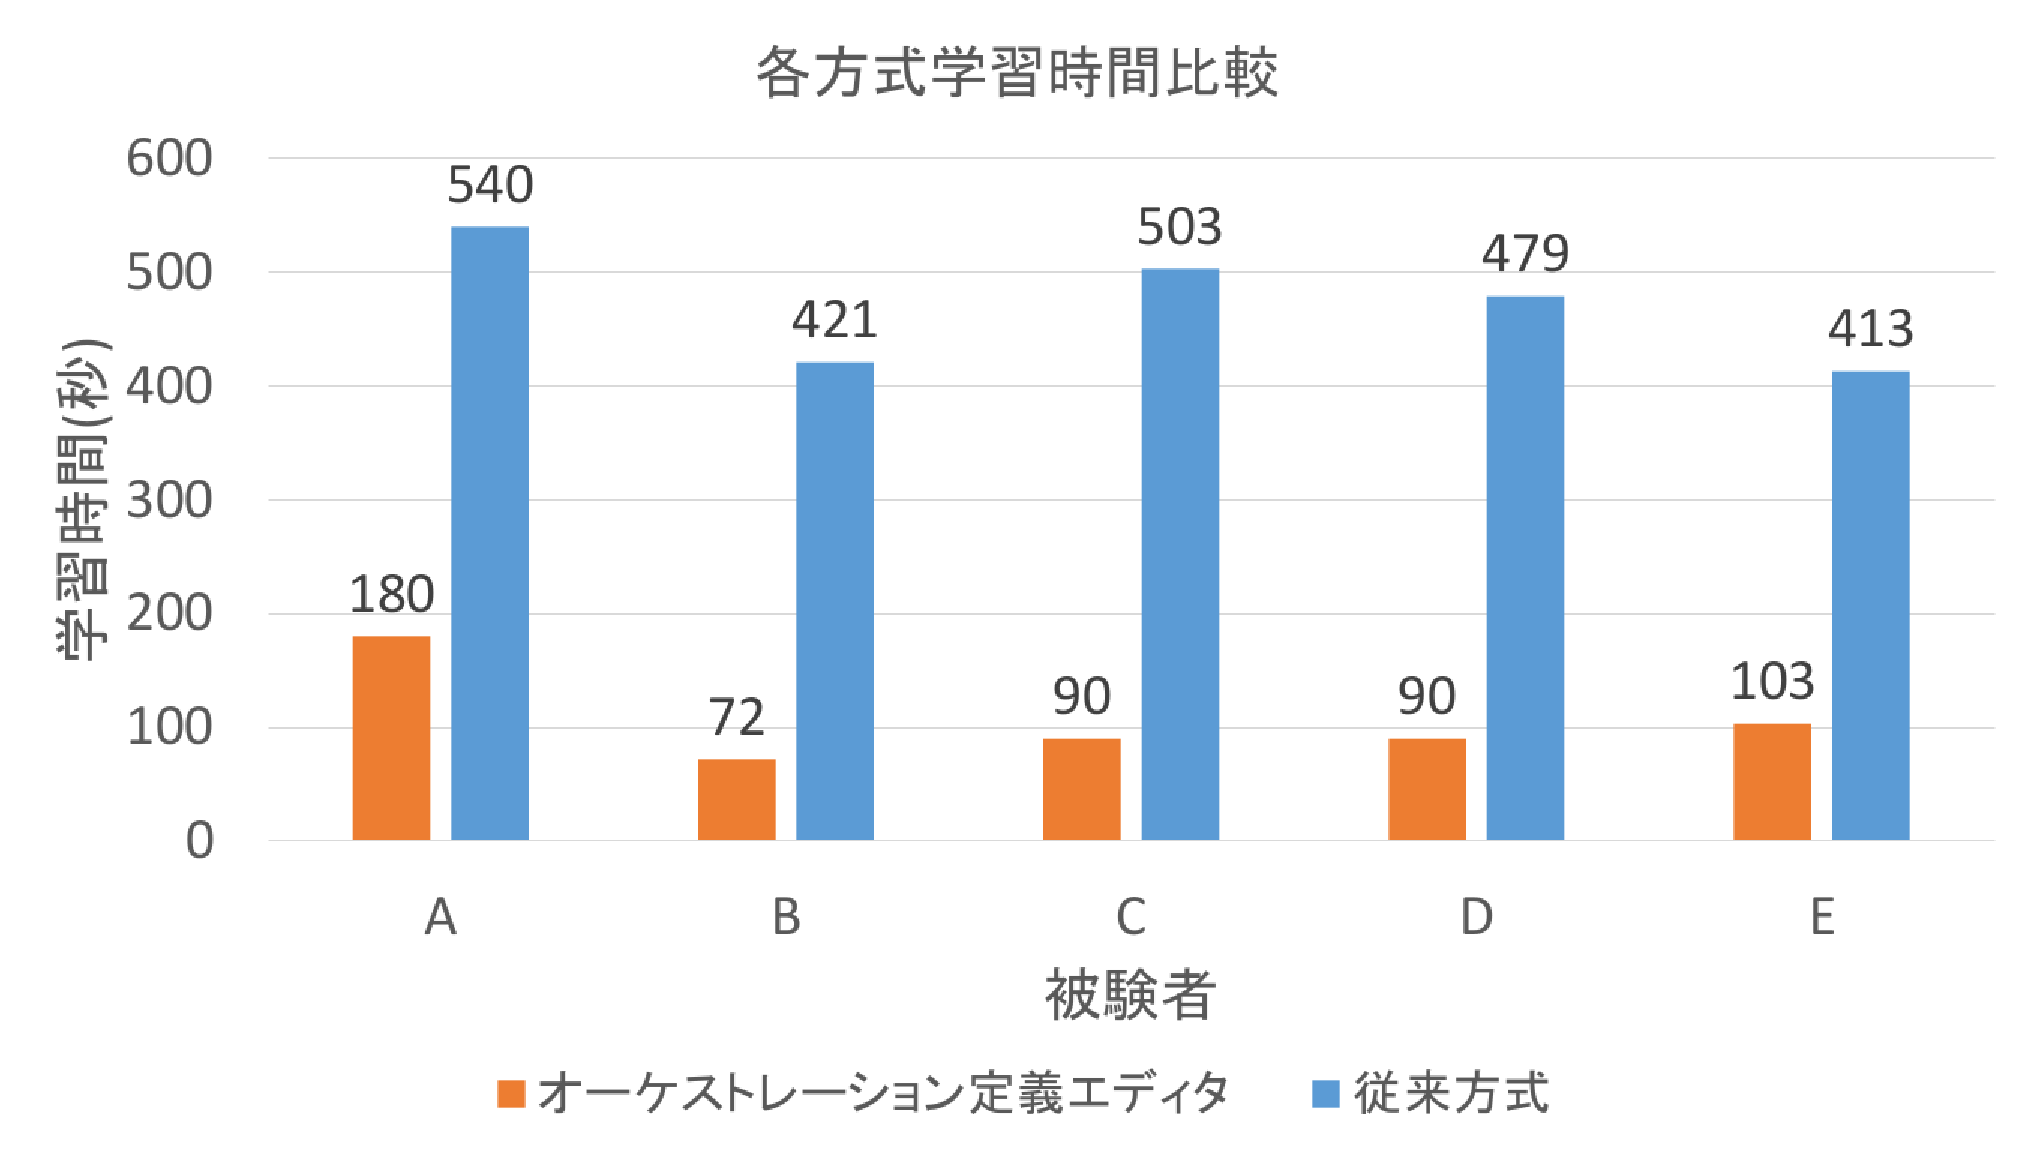
\includegraphics[scale=0.42]{Document/studytime_all.eps}
					\caption{各方式学習時間比較}
					\label{graf:8}
				\end{center}
			\end{figure}
		従来方式ではOpenStackに関する基本的な知識の他に,テンプレートファイル独特の書式について知識が必要であるため,学習すべき項目が多岐に渡ったからだと考えられる.
		
		 一方オーケストレーション定義エディタはボタンとプルダウンメニュー,1箇所のみ手動入力項目に関する説明があるだけで学習すべき項目は従来方式に比べて大幅に少ないからだと考えられる.
		
		 以上のことから,学習時間の面において従来方式よりもオーケストレーション定義エディタのほうが導入が容易であることが示せたと考えられる.
		
		\item[(作成所要時間について)]\mbox{}\\  記録する3つの評価要素のうち,従来方式とオーケストレーション定義エディタ大きく差がでたのが作成所要時間である.従来方式は5人の被験者間で作成所要時間に大きなばらつきがあり,なおかつ作成所要時間そのものも長時間に及んでいた.一方オーケストレーション定義エディタは5人の被験者間で作成所要時間にばらつきはほとんど無く,作成所要時間そのものも従来方式に比べると大幅に少ない.従来方式において最も短い所要時間でテンプレートファイルを作成した被験者Aと最も長い所要時間で作成した被験者Cの比較を図\ref{graf:4}に示す.
		
		\begin{figure}[H]
			\begin{center}
				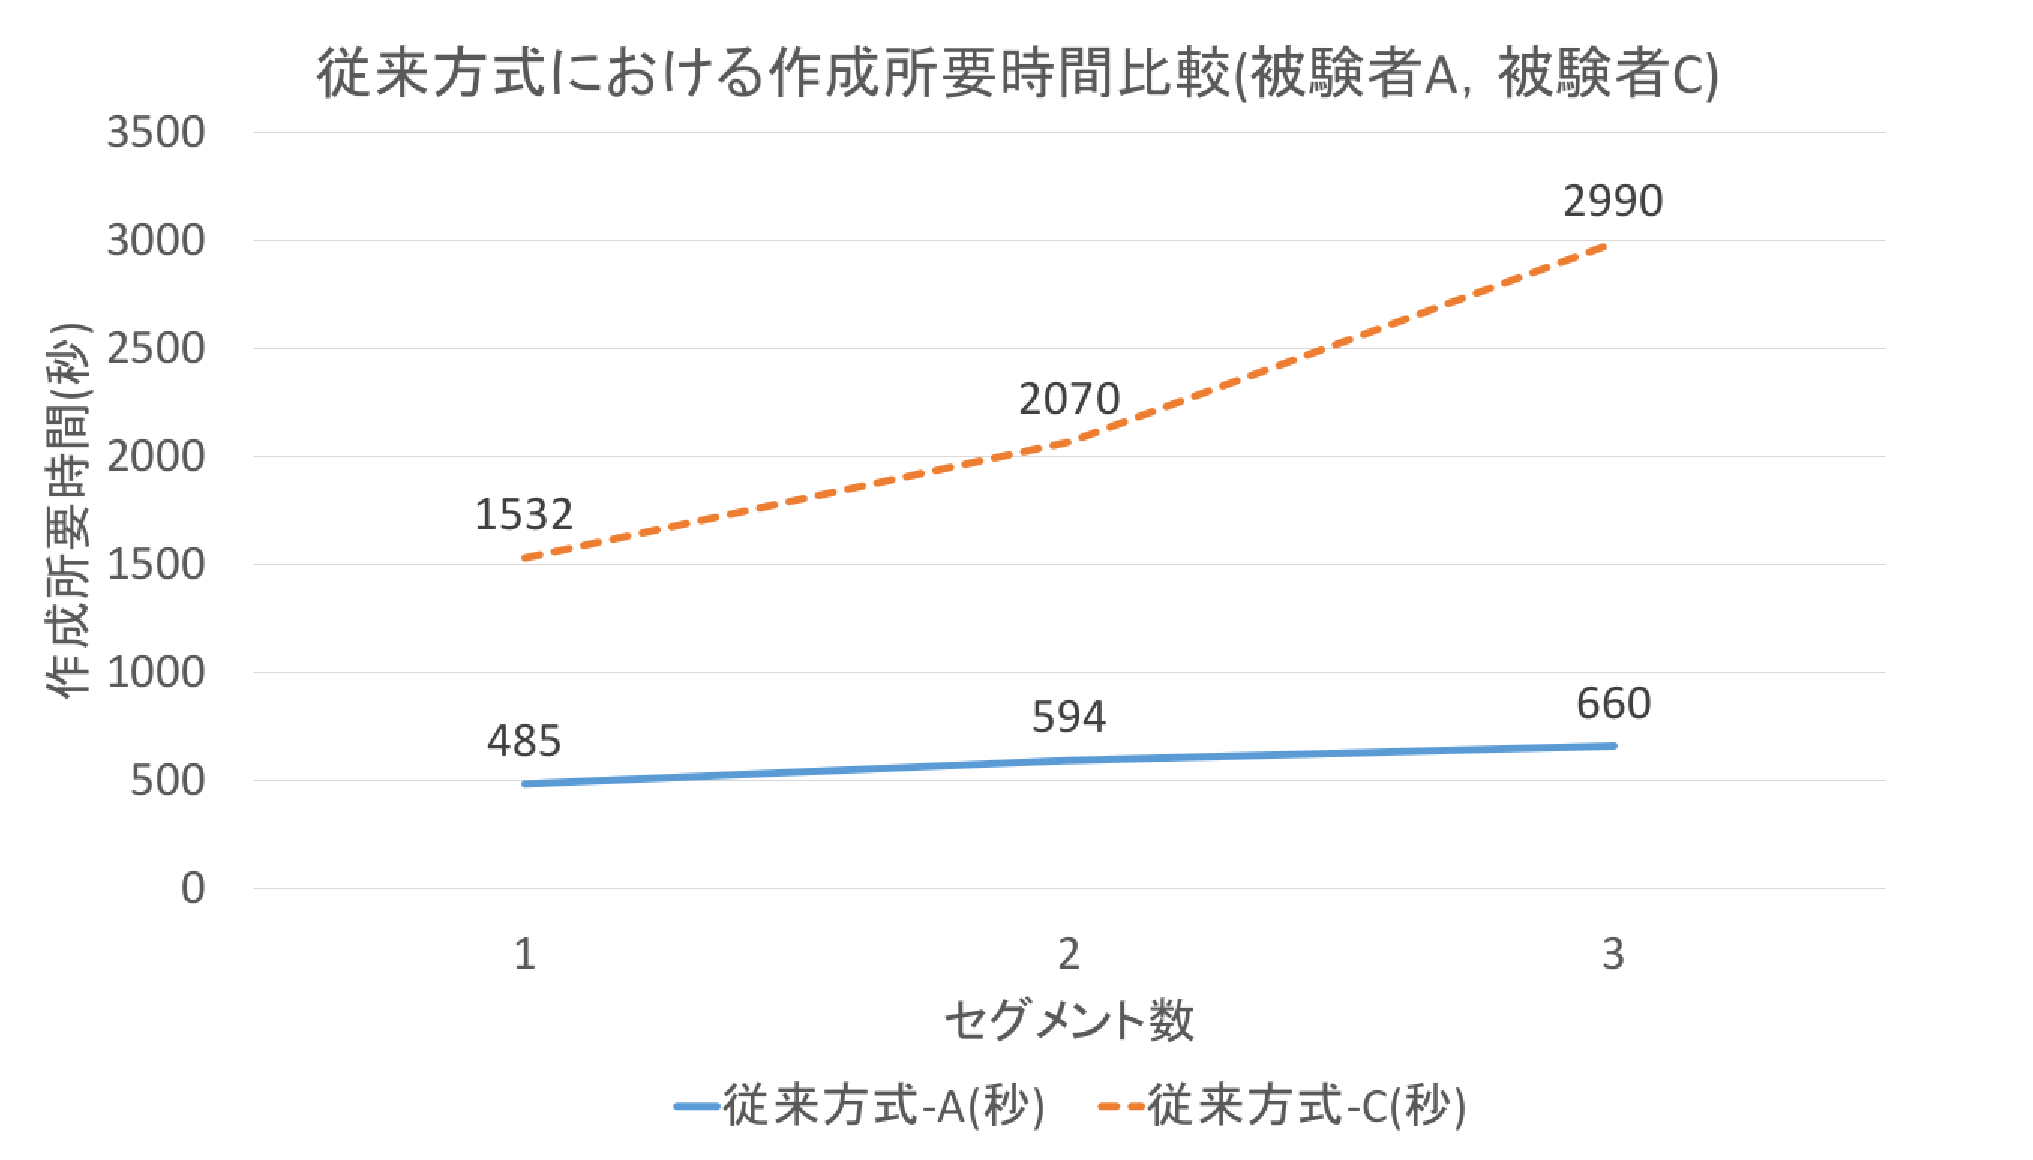
\includegraphics[scale=0.45]{Document/ManualComparisonAC.eps}
				\caption{従来方式における所要時間比較(被験者A,被験者C)}
				\label{graf:4}
			\end{center}
		\end{figure}
		\newpage
		一方同じ被験者Aと被験者Cがオーケストレーション定義エディタを使用して同じ内容のテンプレートファイルを構築した場合,図\ref{graf:5}のような結果が出た.また,構築する内容が似ている(I\hspace{-1pt}I\hspace{-1pt}I),(I\hspace{-1pt}V),(V)を比較した場合図\ref{graf:9}のようになった.
			
		\begin{figure}[H]
			\begin{center}
				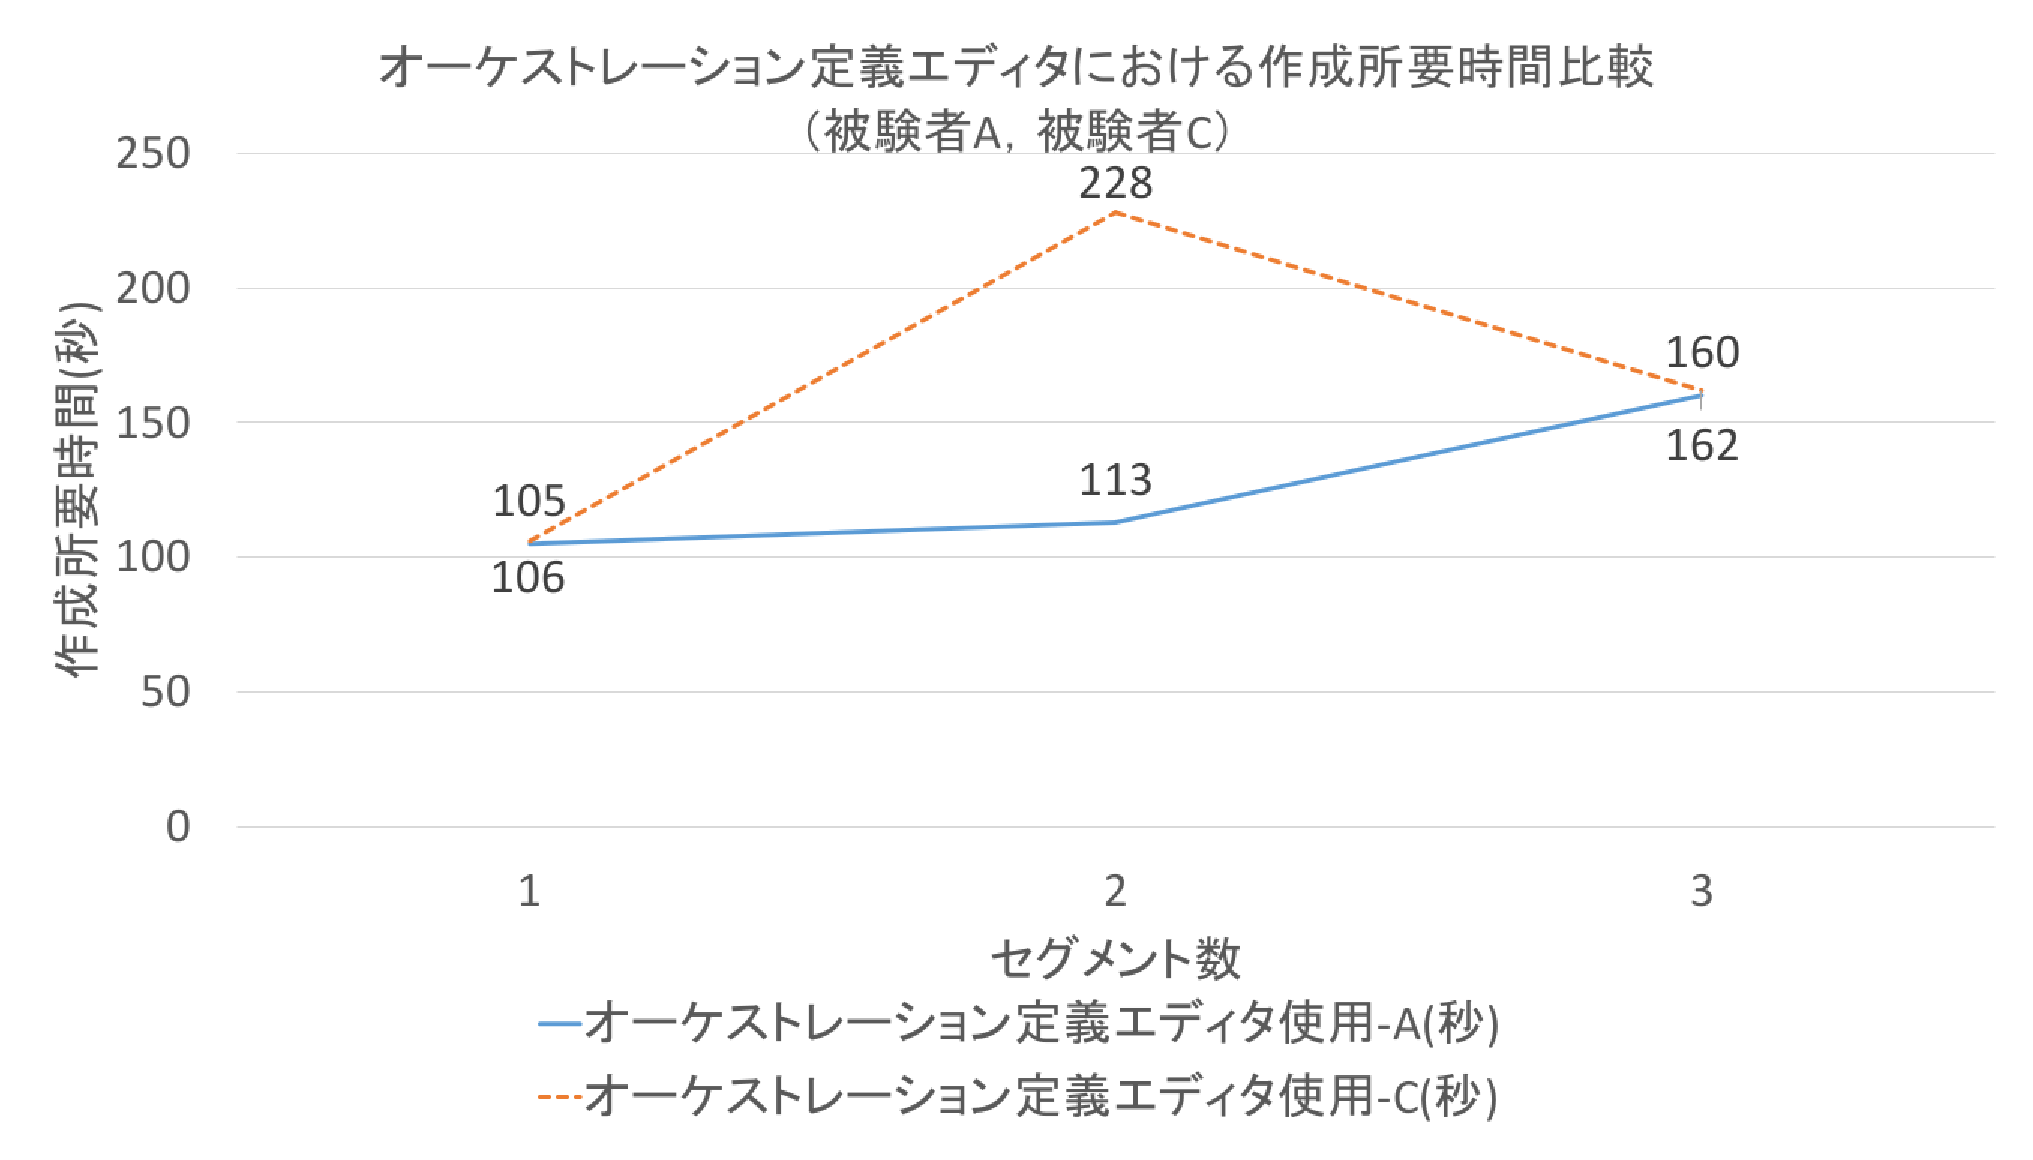
\includegraphics[scale=0.45]{Document/EditorComparisonAC.eps}
				\caption{オーケストレーション定義エディタにおける所要時間比較(被験者A,被験者C)}
				\label{graf:5}
			\end{center}
		\end{figure}
		
		\begin{figure}[H]
			\begin{center}
				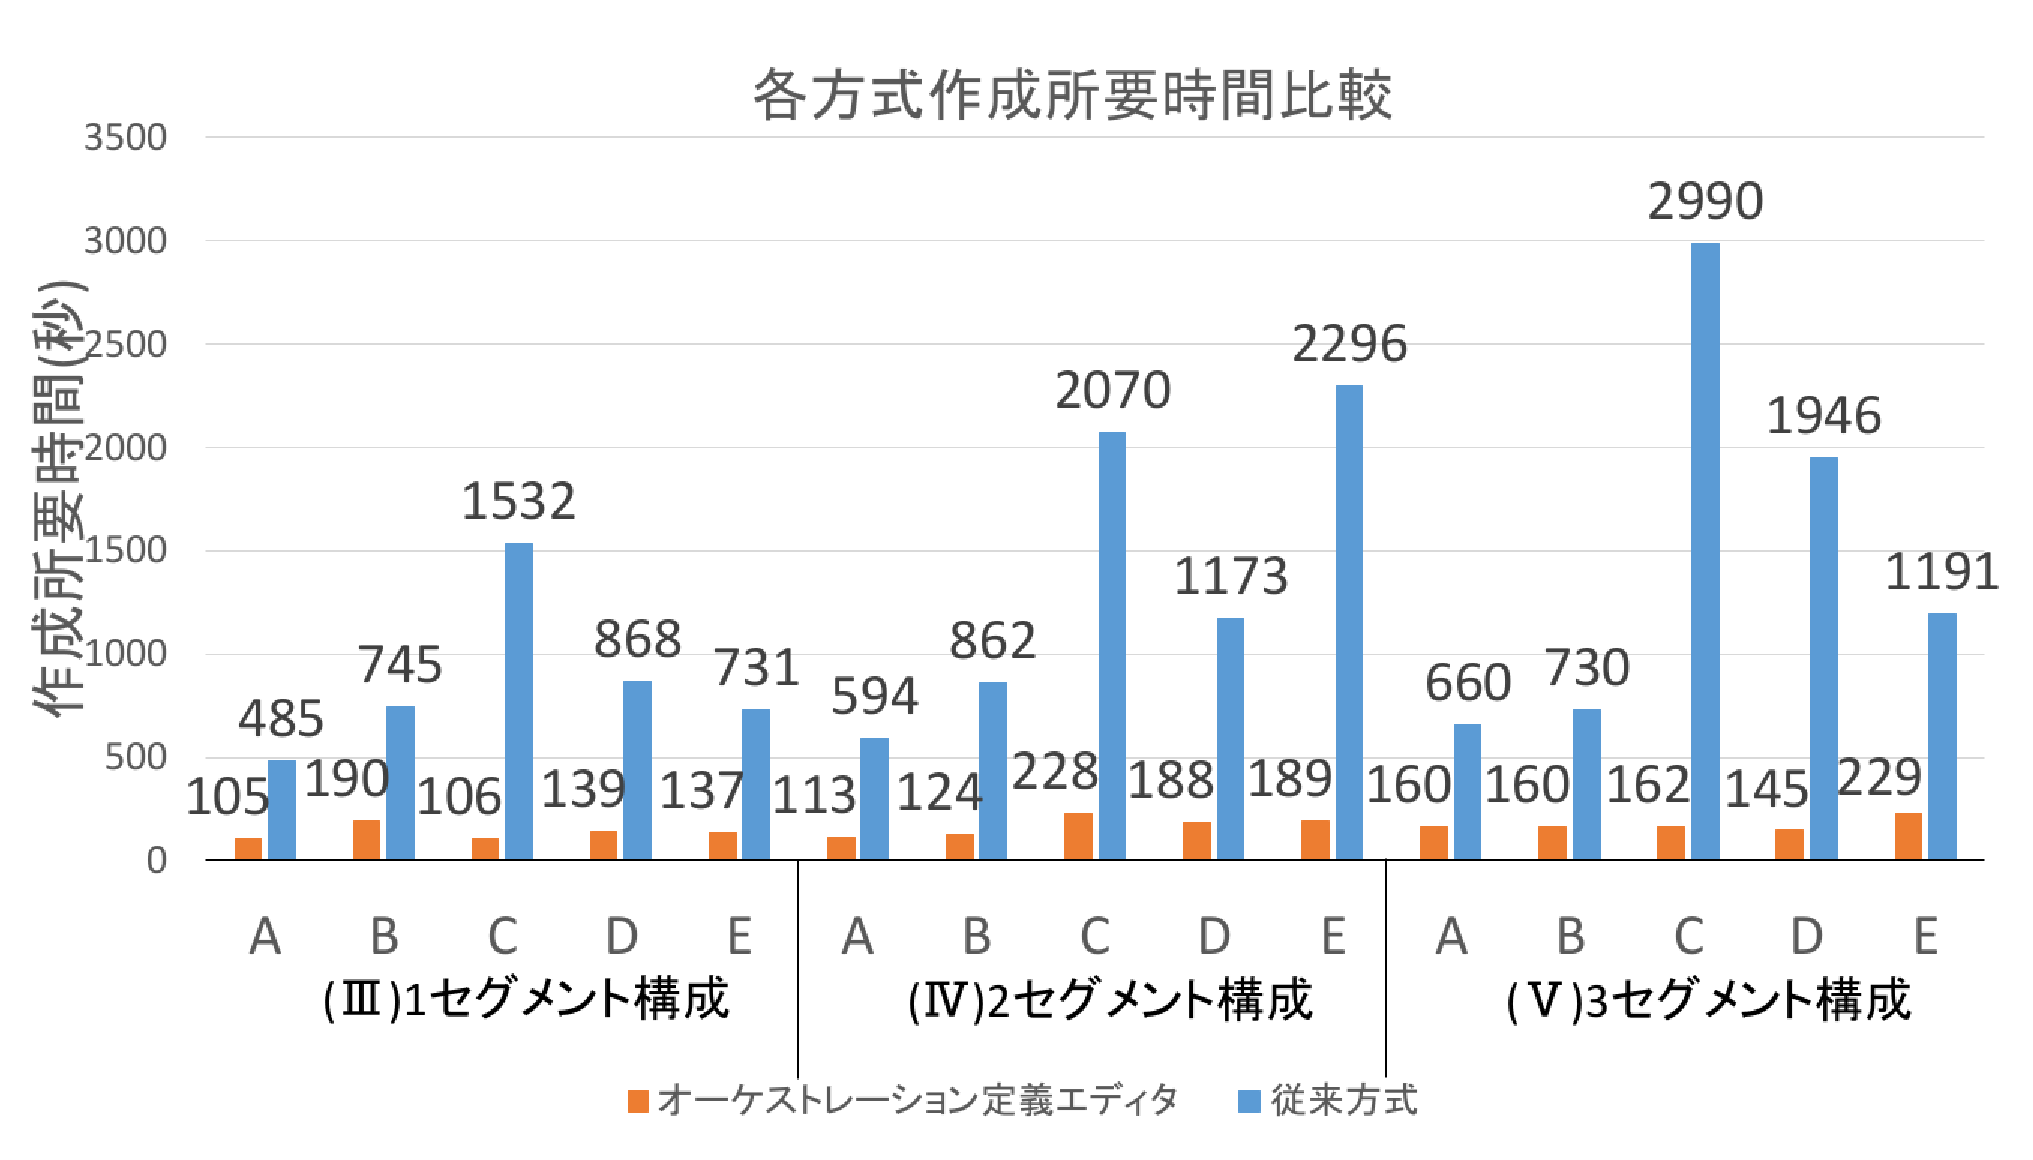
\includegraphics[scale=0.42]{Document/Create_alltime.eps}
				\caption{各方式作成所要時間比較}
				\label{graf:9}
			\end{center}
		\end{figure}
		 従来方式ではテンプレートファイルを作成する場合手動入力で全ての項目を入力しなければならない.入力する際はテンプレートファイル独自の書式に注意しながら入力しなければならず,事前の学習で内容を把握しきっていなければ正確に入力することは困難である.本評価実験において従来方式の事前の学習時間は最長でも540秒であり,被験者たちは10分に満たない学習時間ではテンプレートファイル独自の書式について満足に理解できなかったと考えられる.しかし,従来方式でのテンプレートファイル作成回数が増える毎に従来方式の手動入力に慣れてくる被験者も現れ,システム構成の内容が複雑になっても所要時間の増加幅が少なくなっていった被験者もいた.ただし従来方式の手動入力に慣れることができなかった被験者はシステム構成の内容が複雑になるにつれて所要時間がより多く増加していった.
		
		 以上のことから,従来方式でのテンプレートファイル作成所要時間には個人差が生じやすく,なおかつ作成所要時間は膨大になりがちであるといえる.一方オーケストレーション定義エディタを使用することにより作成所要時間の個人差を無くし,作成所要時間そのものを大幅に削減できる.よって作成所要時間の面でオーケストレーション定義エディタの有用性を示せたと考えられる.
		
		\item[(エラー発生回数について)]\mbox{}\\
		 表\ref{table:6}と\ref{table:7}のとおり,従来方式では,まだテンプレートファイル記述経験の浅いうちに作成したものである(I)作成時のエラー発生回数が最も多い.その後被験者がテンプレートファイル記述に慣れ,エラー発生回数は減少するが,(I\hspace{-1pt}V)においてインスタンス数だけでなくルーター(ネットワーク)数を増加,つまり新たな追加記述要素が加わることでエラー発生回数は増加した.被験者5人が従来方式にて発生させたエラー回数について図\ref{graf:6}に示す.
		\vspace{-2.8mm}
		\begin{figure}[H]
			\begin{center}
				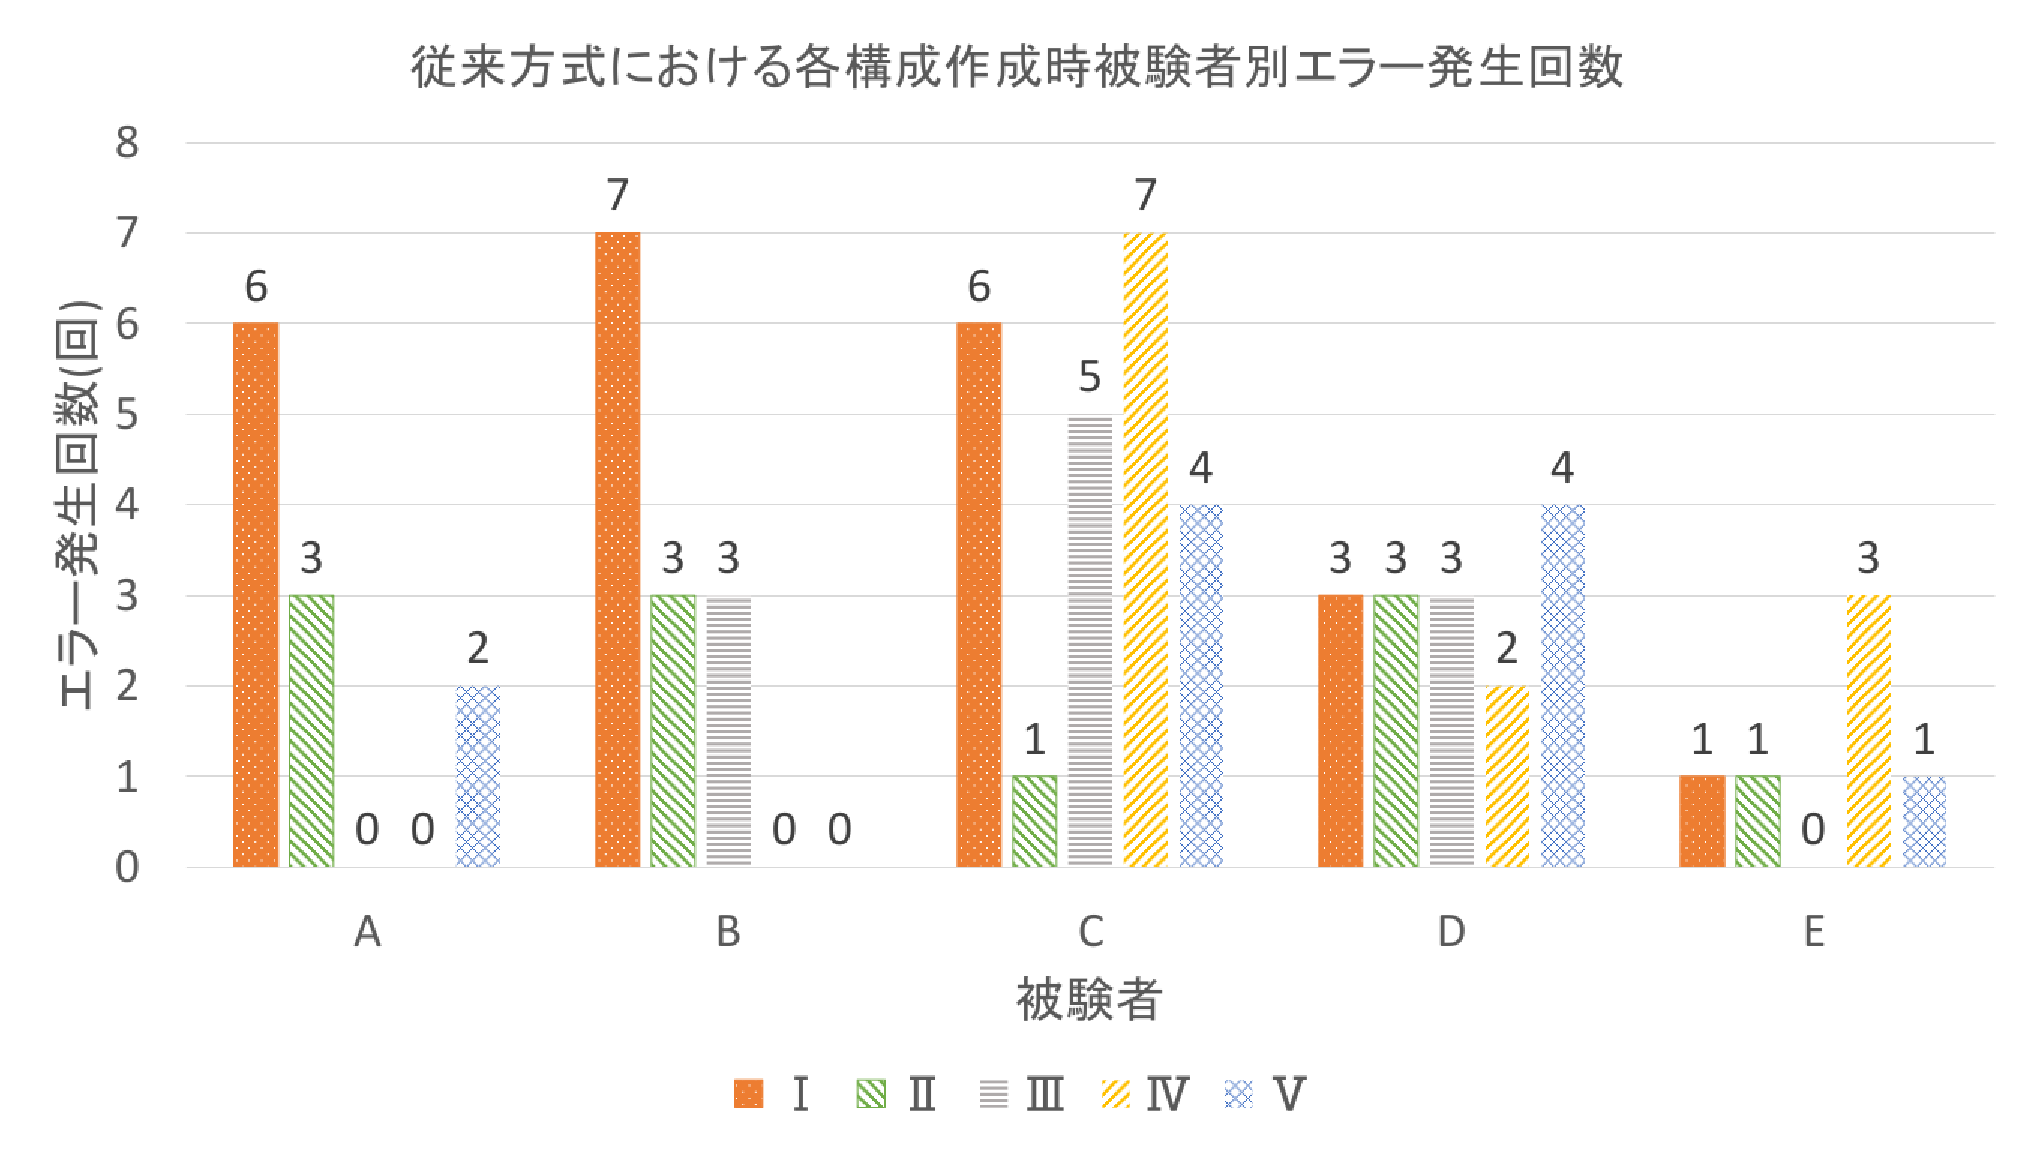
\includegraphics[scale=0.45]{Document/TemplateFile_ErrorGraf.eps}
				\caption{従来方式における各構成作成時被験者別エラー発生回数}
				\label{graf:6}
			\end{center}
		\end{figure}
		 一方オーケストレーション定義エディタを使用した際は表\ref{table:7}のとおりテンプレートファイル作成時にエラーは発生しなかった.これは,入力される内容が決まっている項目は予め文字列データとして保存,出力時に所定の位置へ出力をしており,尚且つテンプレートファイル毎に入力内容が異なるものに関してはプルダウンメニューを用いて選択肢を用意し利用者に選択させ決定後にテンプレートファイルに出力しているので,利用者が記述内容をミスし得ない状態だからである.
		
		 よって,利用者はテンプレートファイルに関する専門知識を意識すること無く容易且つ正確にテンプレートファイルを作成できるといえる.
	\end{description}
\chapter{おわりに}
	\section{研究のまとめ}
	本研究では,OpenStack内コンポーネントであるHeatを使用したシステム定義をテンプレートファイルに記述するうえで問題点となっていた「膨大なテキスト記述量」と,「構成情報把握のしづらさ」,「テンプレートファイルの書式の複雑さ」を解決するためにオーケストレーション定義エディタを提案し,実現した.
	
	操作インターフェイスをGUIにすることにより,構築中でも構成内容を把握できるようになった.複雑な書式でテキストのみで入力されたテンプレートファイルの構成内容を,GUIを用いて可視化させることができた.これにより「構成情報の把握しづらさ」を解決した.
	
	オーケストレーション定義エディタでは,構築毎に入力内容が変わらない項目は予め文字列データとして保管しておく.これらの内容は出力時に自動で適切なデータだけをテンプレートファイルへ出力する.一方構築毎に内容が変わる項目は専用のデータ保管用Classを用意し,利用者から入力された内容を保管する.尚,保管用Classへデータを保存する項目は詳細入力画面とよばれる画面でプルダウンメニューにより選択肢を提供される.その後出力時にテンプレートファイルへ出力される.これらにより,従来テキストで記述していた内容をほとんどプルダウンメニューによる選択と自動入力で記述できるようになり,利用者はテンプレートファイルの複雑な書式を意識すること無く,プルダウンメニューを選択するだけで項目の入力が可能となった.これにより問題点である「テンプレートファイルの書式の複雑さ」と「膨大なテキスト記述量」を解決できた.
	
	第4章の評価実験により,オーケストレーション定義エディタを用いることによりテンプレートファイル作成時のエラー発生回数を激減させることができ,自動入力等の補助によりテンプレートファイル作成所要時間も大幅に減少させることができた.また,オーケストレーション定義エディタを使用してテンプレートファイルを作成した際,5人の被験者の各作成所要時間に大きな差が開いていなかった.以上のことから,利用者の能力に依存すること無く短時間かつ容易で正確にテンプレートファイルを構築し,仮想環境を構築できることがわかった.
	
	つまり,オーケストレーション定義エディタの実現によりテンプレートファイルに関する専門的な知識を意識させること無く,利用者の能力に左右されること無く短時間かつ正確,そして容易にテンプレートファイルを作成可能であることが示せた.
	
	また,オーケストレーション定義エディタはテンプレートファイルへの記述補助エディタであるため,基本的に記述させる内容を追加することは容易である.つまり,Heatの機能内であれば機能や動作を追加できるので,拡張性は高いといえる.
	\section{今後の課題}
	オーケストレーション定義エディタの問題点として,起動するインスタンスを追加する際,1つずつしか追加できない点があげられる.これでは,仮に同じ内容のインスタンスを複数個起動させようとした場合でも,起動するインスタンスの数だけ同じ内容の記述をそれぞれの詳細入力画面で繰り返さなければならない.これを改善する案として詳細入力画面に「起動させるインスタンス数」という項目を追加し,同時に起動させるインスタンス数を指定できるようにする方法が挙げられる.この機能を追加することにより,同じ内容のインスタンスを複数個起動させたい場合であれば現時点のオーケストレーション定義エディタでの操作よりも操作回数を減少させることができ,テンプレートファイル作成所要時間も減少させることができる.
	

%% 謝辞 %%%%%%%%%%%%%%%%%%%%%%%%%%%%%%%%%%%%%%%%%%%%%%%%%%%%%%%%%%%%%%%%

\begin{acknowledgement}
本研究を進めるにあたり,研究指導及び論文審査の主査として,横山和俊教授には多くのご指導を頂きました.また,研究室での活動だけではなく就職活動や社会人としての心構えについて数多くのご指導を頂きました.心より感謝致します.本研究の副査をお引き受けいただき,数々のご質問,ご指摘を頂きました情報学群 岩田誠教授と鵜川始陽准教授に心より感謝致します.

分散処理OS研究室の同期である大崎康平君,別役速斗君,小池主馬君には,日頃の勉学をはじめ各種研究室内イベントや卒業研究でたくさんお世話になりました.ありがとうございました.また,分散処理OS研究室の先輩である畑翔太氏には勉学や研究内容について数多くの手助けをしていただきました.ありがとうございました.後輩である松岡亨一君,川村郁哉君,手塚詞央里さん,濱田哲郎君,船越勇樹君,本研究の評価実験への協力をはじめとする,日頃の様々な場面において力になってくれて本当にありがとうございました.

最後に,様々な側面から私を見守り,支えてくださった家族に心から感謝します.
%\input{acknowledgement.tex}
\end{acknowledgement}

%% 参考文献 %%%%%%%%%%%%%%%%%%%%%%%%%%%%%%%%%%%%%%%%%%%%%%%%%%%%%%%%%%%%

\begin{thebibliography}{99}
%\input{bibliography.tex}
\bibitem{bib:1}総務省 平成27年度版 情報通信白書 第5章第2節「ICT産業のグローバルトレンド」 				\url{http://www.soumu.go.jp/johotsusintokei/whitepaper/ja/h27/pdf/index.html}
\bibitem{bib:2}IBMクラウド・コンピューティング:IaaSとは-Japan
\url{http://www.ibm.com/cloud-computing/jp/ja/what-is-iaas.html}
\bibitem{bib:3}OpenStack
\url{https://www.openstack.org}
\bibitem{bib:4}OpenStackCloudSoftware Heat Documentation
\url{http://docs.openstack.org/developer/heat/index.html}
\end{thebibliography}

%% 付録 %%%%%%%%%%%%%%%%%%%%%%%%%%%%%%%%%%%%%%%%%%%%%%%%%%%%%%%%%%%%%%%%

%\appendix

%\chapter{}
%\input{appendex1.tex}

%\chapter{}
%\input{appendex2.tex}

\end{document}
